\section{Bài toán Riemann và Cấu trúc sóng}
\subsection{Giới thiệu chung}

Bài toán ống sốc của Sod, được giới thiệu bởi Gary A. Sod vào năm 1978, là một trường hợp kiểm thử (test case) kinh điển trong động lực học chất lưu tính toán (CFD). Đây là một dạng cụ thể của \textbf{bài toán Riemann} cho hệ phương trình Euler đối với khí lý tưởng. 

Mục đích chính của bài toán là đánh giá khả năng của các thuật toán số trong việc bắt giữ các gián đoạn vật lý như sóng sốc và gián đoạn tiếp xúc, đồng thời xử lý các vùng biến đổi liên tục như sóng loãng.

Xét một ống dài được chia thành hai phần bằng nhau bởi một màng ngăn, với hai bên màng ngăn được bơm khí với mật độ và áp suất khác nhau:
$$
\rho_L = 1.0, \quad \rho_R = 0.125, \quad p_L = 1.0, \quad p_R = 0.1.
$$
và vận tốc ban đầu ở cả hai bên màng ngăn đều bằng 0.

\begin{figure}[H]
\centering
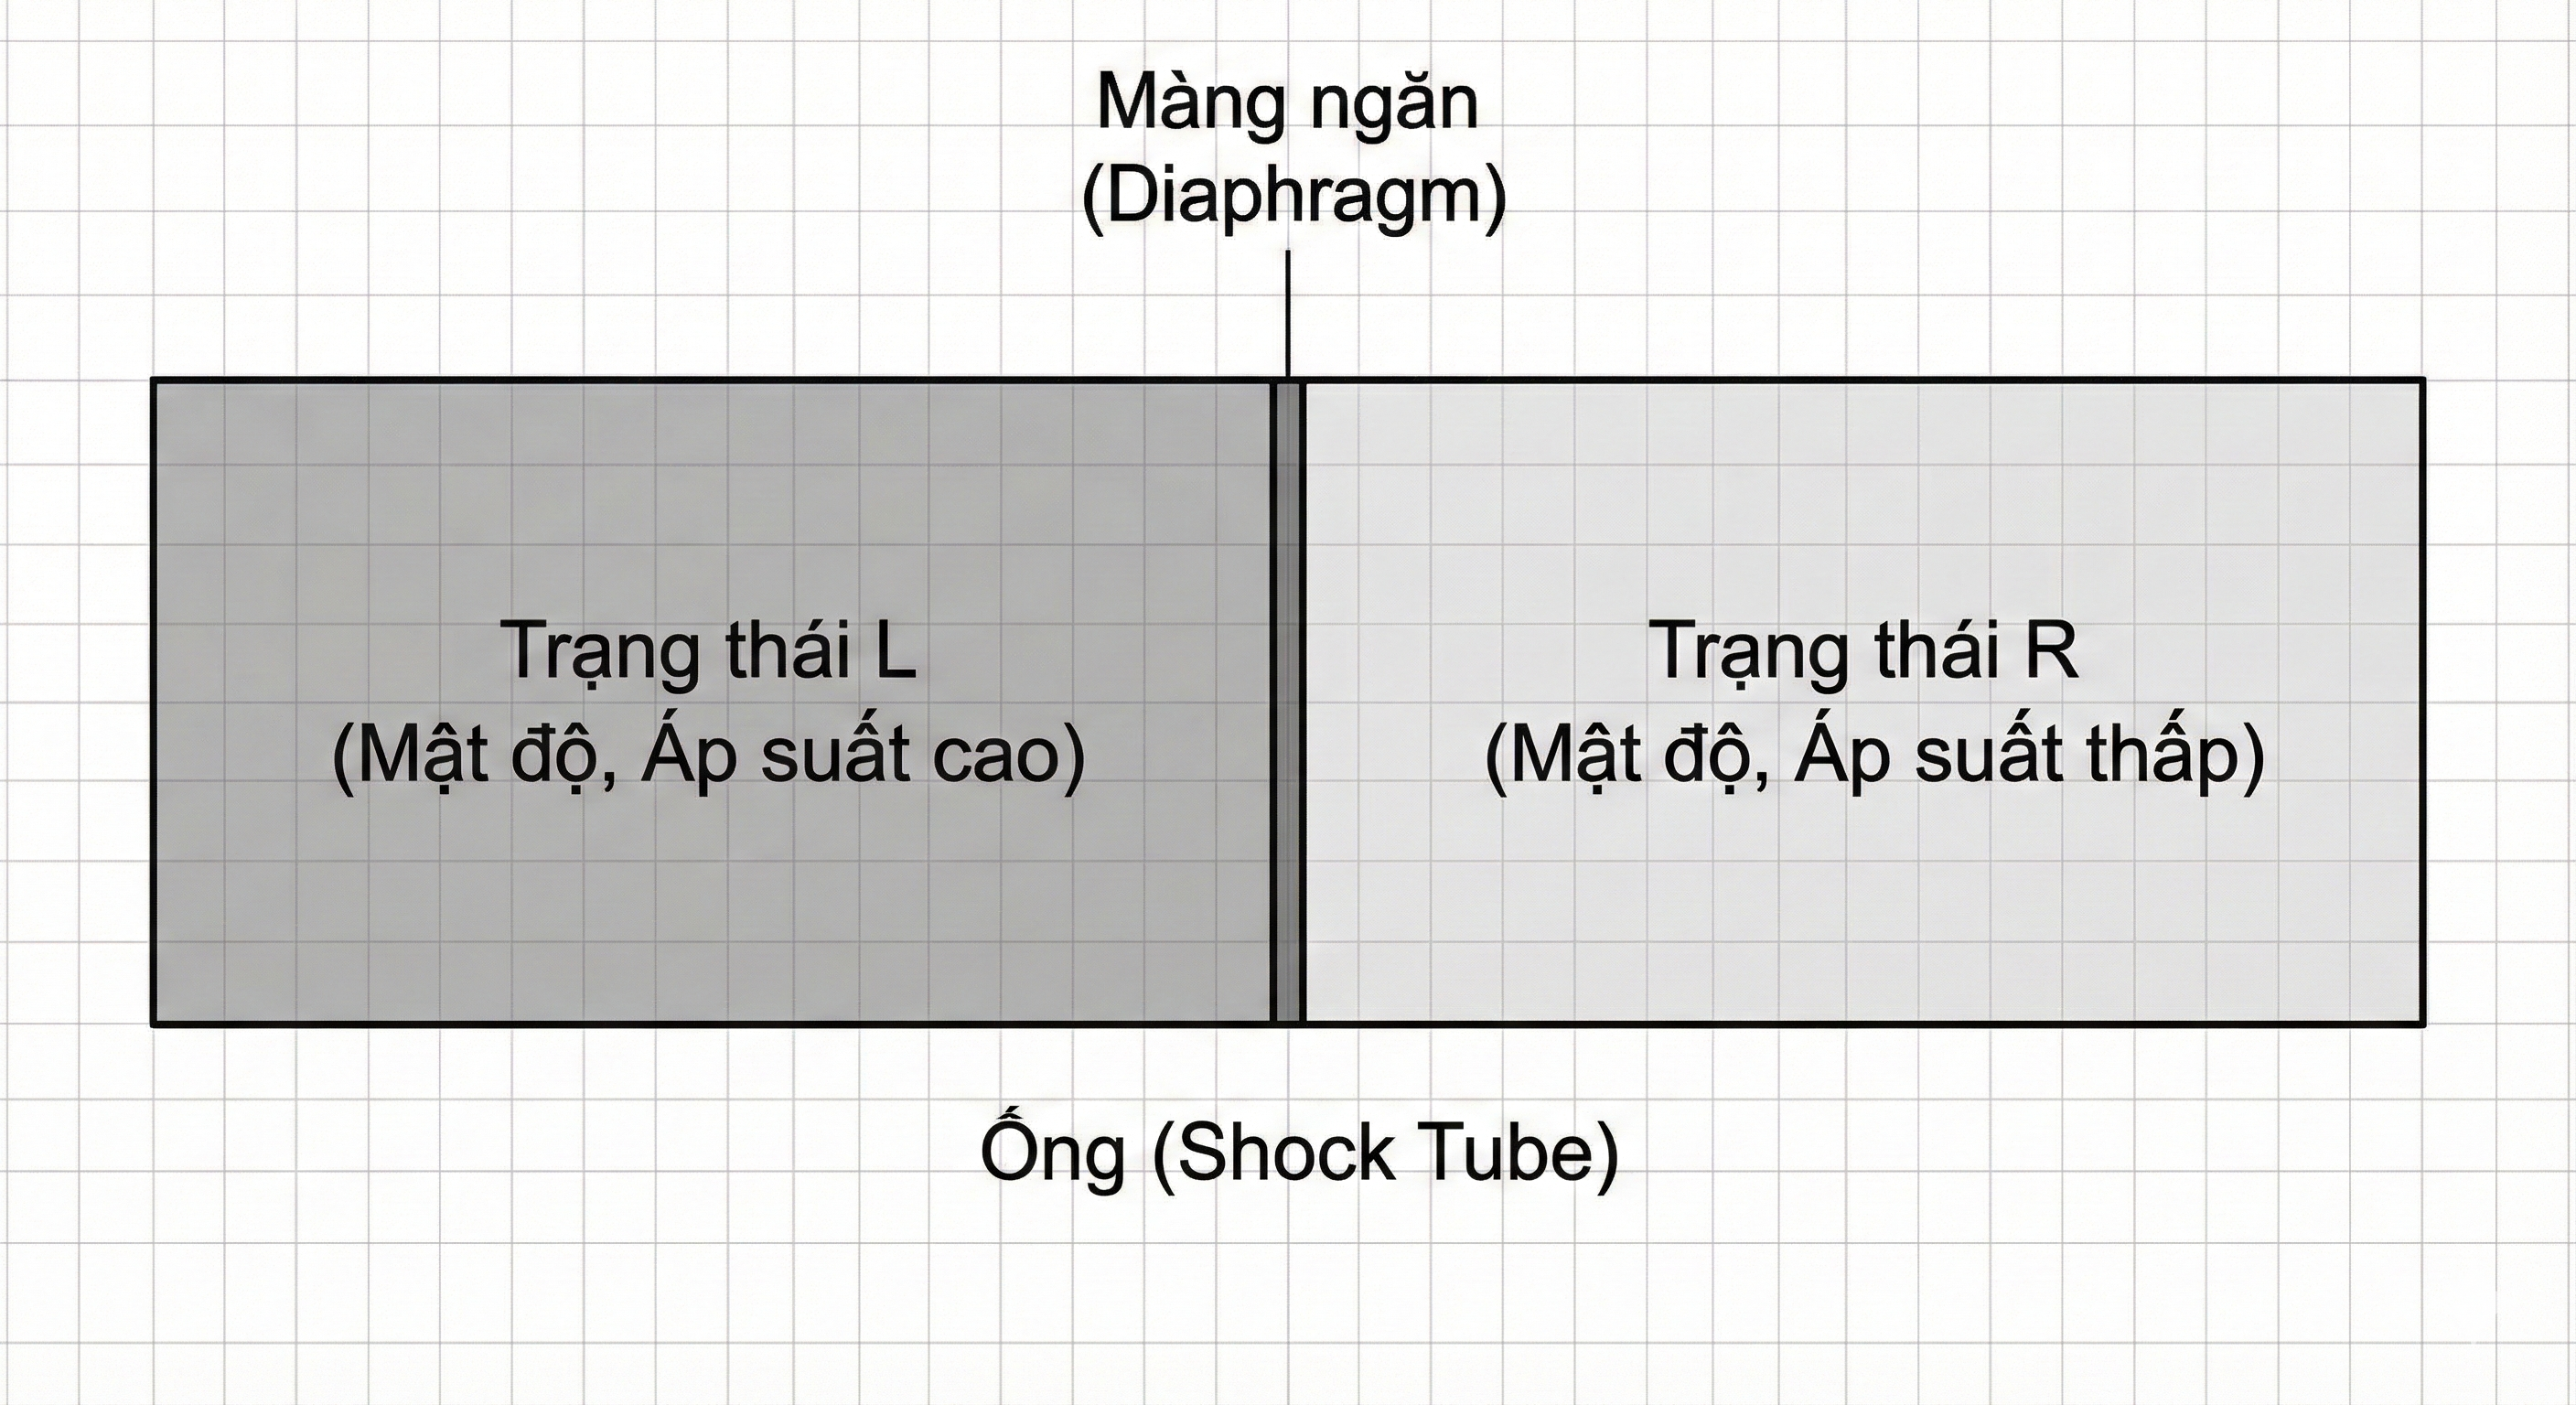
\includegraphics[width=0.8\textwidth]{tube.png}
\caption{Sơ đồ bài toán ống sốc Sod}
\label{fig:sod_tube}
\end{figure}

Bài toán trên có thể được giải thông qua việc giải phương trình sau:

\begin{equation*}
    \frac{\partial \mathbf{W}}{\partial t} + \frac{\partial \mathbf{F}(\mathbf{W})}{\partial x} = 0
\end{equation*}

Các vector cột trong phương trình trên được định nghĩa cụ thể thông qua các biến vật lý:

\begin{equation*}
    \mathbf{W} = \begin{bmatrix}
    w_1 \\
    w_2 \\
    w_3
    \end{bmatrix} = \begin{bmatrix}
    \rho \\
    \rho u \\
    \rho E
    \end{bmatrix}, \quad
    \mathbf{F}(\mathbf{W}) = \begin{bmatrix}
    f_1 \\
    f_2 \\
    f_3
    \end{bmatrix} = \begin{bmatrix}
    \rho u \\
    \rho u^2 + p \\
    u(\rho E + p)
    \end{bmatrix}
\end{equation*}

Với $\rho$ là mật độ, $u$ là vận tốc, $p$ là áp suất và $E$ là tổng năng lượng trên một đơn vị thể tích. Mối liên hệ giữa các đại lượng được xác định qua phương trình trạng thái khí lý tưởng:
\begin{equation*}
E = \frac{p}{\gamma - 1} + \frac{1}{2}\rho u^2
\end{equation*}
Thông thường, hệ số nhiệt dung đẳng áp được chọn là $\gamma = 1.4$.


\subsection{Phương pháp giải nghiệm chính xác}

Ta xét bài toán Riemann đối với hệ phương trình Euler 1 chiều cho khí lý tưởng với tỷ số nhiệt dung $\gamma$. Điều kiện đầu tại thời điểm $t=0$ được cho bởi trạng thái gián đoạn tại vị trí $x_0$:
\begin{equation*}
    W(x, 0) = \begin{cases} 
    W_L = (\rho_L, u_L, p_L)^T & \text{nếu } x < x_0 \\
    W_R = (\rho_R, u_R, p_R)^T & \text{nếu } x > x_0
    \end{cases}
\end{equation*}
Giả sử rằng $p_L > p_R$, khi đó cấu trúc nghiệm của bài toán sẽ bao gồm: một sóng giãn (Rarefaction wave) lan truyền về phía trái, một gián đoạn tiếp xúc (Contact discontinuity) ở giữa, và một sóng xung kích (Shock wave) lan truyền về phía phải. Cấu trúc này chia mặt phẳng $x-t$ thành 4 vùng cơ bản: vùng trái ($L$), vùng sao trái ($L^*$), vùng sao phải ($R^*$), và vùng phải ($R$) (xem ảnh minh họa bên dưới).

\begin{figure}[H]
\centering
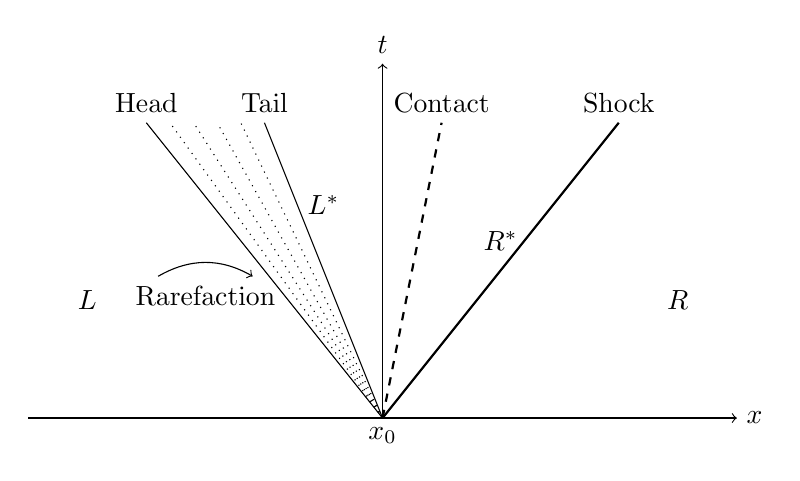
\begin{tikzpicture}[scale=1.5]
    % Draw axes
    \draw[->] (-3,0) -- (3,0) node[right] {$x$};
    \draw[->] (0,0) -- (0,3) node[above] {$t$};
    
    % Origin label
    \node[below] at (0,0) {$x_0$};
    
    % Rarefaction Fan (Left)
    \draw (0,0) -- (-2,2.5) node[above] {Head};
    \draw (0,0) -- (-1,2.5) node[above] {Tail};
    \foreach \i in {-1.8, -1.6, ..., -1.2}
        \draw[dotted] (0,0) -- (\i, 2.5);
        
    % Contact Discontinuity (Middle)
    \draw[dashed, thick] (0,0) -- (0.5,2.5) node[above] {Contact};
    
    % Shock Wave (Right)
    \draw[thick] (0,0) -- (2,2.5) node[above] {Shock};
    
    % Labels for regions
    \node at (-2.5, 1) {$L$};
    \node at (-0.5, 1.8) {$L^*$};
    \node at (1, 1.5) {$R^*$};
    \node at (2.5, 1) {$R$};
    
    % Arrow indicating expansion fan
    \draw[->] (-1.9, 1.2) to[bend left] (-1.1, 1.2);
    \node[below] at (-1.5, 1.2) {Rarefaction};

\end{tikzpicture}
\caption{Cấu trúc nghiệm bài toán Riemann trong mặt phẳng $x-t$ với $p_L > p_R$}
\label{fig:riemann_structure}
\end{figure}

Để tìm nghiệm chính xác $W(x,t)$ tại một thời điểm $t > 0$, ta thực hiện theo các bước sau:

\textbf{Bước 1: Thiết lập phương trình cho áp suất vùng sao ($p^*$)}

Do vận tốc $u$ và áp suất $p$ liên tục qua gián đoạn tiếp xúc, ta có $u_L^* = u_R^* = u^*$ và $p_L^* = p_R^* = p^*$. Ta thiết lập mối quan hệ giữa vận tốc và áp suất qua các sóng để tìm $p^*$.

Hàm vận tốc qua sóng giãn bên trái ($L \to L^*$) được xác định bởi bất biến Riemann:
\begin{equation*}
    u_L^*(p) = u_L + \frac{2a_L}{\gamma-1}\left[ 1 - \left( \frac{p}{p_L} \right)^{\frac{\gamma-1}{2\gamma}} \right]
\end{equation*}
trong đó $a_L = \sqrt{\gamma p_L / \rho_L}$ là vận tốc âm thanh tại miền trái.

Hàm vận tốc qua sóng xung kích bên phải ($R \to R^*$) được xác định bởi hệ thức Rankine-Hugoniot:
\begin{equation*}
    u_R^*(p) = u_R + (p - p_R) \sqrt{\frac{A_R}{p + B_R}}
\end{equation*}
với các hằng số $A_R = \frac{2}{(\gamma+1)\rho_R}$ và $B_R = \frac{\gamma-1}{\gamma+1}p_R$.

Tại vùng sao, vận tốc phải cân bằng, tức là $u_L^*(p^*) = u_R^*(p^*)$. Do đó, ta cần tìm nghiệm $p^*$ của phương trình phi tuyến:
\begin{equation*}
    f(p) = u_L^*(p) - u_R^*(p) = 0
\end{equation*}

\textbf{Bước 2: Giải lặp tìm áp suất $p^*$}

Do phương trình $f(p)=0$ là phi tuyến, ta sử dụng phương pháp lặp Newton-Raphson để tìm nghiệm gần đúng với độ chính xác mong muốn. Giá trị khởi tạo $p_{(0)}$ có thể chọn bằng trung bình cộng hoặc xấp xỉ tuyến tính (Two-Rarefaction approximation):
\begin{equation*}
    p_{(0)} = \frac{p_L + p_R}{2} \quad \text{hoặc} \quad p_{(0)} = \left[ \frac{a_L + a_R - \frac{\gamma-1}{2}(u_R - u_L)}{\frac{a_L}{p_L^{(\gamma-1)/(2\gamma)}} + \frac{a_R}{p_R^{(\gamma-1)/(2\gamma)}}} \right]^{\frac{2\gamma}{\gamma-1}}
\end{equation*}

Công thức lặp tại bước $k$:
\begin{equation*}
    p_{(k+1)} = p_{(k)} - \frac{f(p_{(k)})}{f'(p_{(k)})}
\end{equation*}

trong đó đạo hàm $f'(p)$ được tính bằng:
\begin{equation*}
    f'(p) = \frac{\partial u_L^*}{\partial p} - \frac{\partial u_R^*}{\partial p}
\end{equation*}
Quá trình lặp dừng lại khi sai số tương đối $\frac{|p_{(k+1)} - p_{(k)}|}{p_{(k)}} < \epsilon$, với $\epsilon$ là sai số cho phép (ví dụ $10^{-6}$).

\textbf{Bước 3: Xác định các biến trạng thái trong vùng sao}

Sau khi tìm được áp suất hội tụ $p^*$, ta tính vận tốc dòng $u^*$ bằng cách thay $p^*$ vào phương trình (2) hoặc (3). Tiếp theo, ta xác định khối lượng riêng tại hai phía của gián đoạn tiếp xúc:

Tại vùng sao trái ($L^*$), sử dụng quan hệ đẳng entropy:
\begin{equation*}
    \rho_L^* = \rho_L \left( \frac{p^*}{p_L} \right)^{1/\gamma}
\end{equation*}

Tại vùng sao phải ($R^*$), sử dụng quan hệ Rankine-Hugoniot:
\begin{equation*}
    \rho_R^* = \rho_R \left( \frac{1 + \beta (p^*/p_R)}{\beta + (p^*/p_R)} \right), \quad \text{với } \beta = \frac{\gamma+1}{\gamma-1}
\end{equation*}

Năng lượng tổng của các vùng sao được tính theo:
\begin{equation*}
    E_L^* = \frac{p^*}{\gamma-1} + \frac{1}{2}\rho_L^* (u^*)^2, \quad E_R^* = \frac{p^*}{\gamma-1} + \frac{1}{2}\rho_R^* (u^*)^2
\end{equation*}

\textbf{Bước 4: Tổng hợp nghiệm tại điểm $(x,t)$}

Cuối cùng, ta xác định giá trị của $W(x,t)$ dựa trên vị trí của $x$ so với các đặc trưng sóng. Các vận tốc truyền sóng được tính như sau:
\begin{itemize}
    \item Vận tốc đầu sóng giãn: $S_{HL} = u_L - a_L$
    \item Vận tốc đuôi sóng giãn: $S_{TL} = u^* - a_L^*$, với $a_L^* = \sqrt{\gamma p^*/\rho_L^*}$
    \item Vận tốc gián đoạn tiếp xúc: $S_{Contact} = u^*$
    \item Vận tốc sóng xung kích: $S_{Shock} = u_R + a_R \sqrt{\frac{\gamma+1}{2\gamma}\frac{p^*}{p_R} + \frac{\gamma-1}{2\gamma}}$
\end{itemize}

\textbf{Lưu ý về gián đoạn tiếp xúc:} Gián đoạn tiếp xúc di chuyển với vận tốc $u^*$ và duy trì sự liên tục của áp suất và vận tốc nhưng cho phép sự gián đoạn trong mật độ. Qua gián đoạn này, $p_L^* = p_R^* = p^*$ và $u_L^* = u_R^* = u^*$, nhưng $\rho_L^* \neq \rho_R^*$.

Khi đó, nghiệm tại vị trí $x$ và thời điểm $t$ là:
\begin{equation*}
    W(x,t) = \begin{cases} 
    W_L & \text{nếu } x/t < S_{HL} \\
    W_{fan} & \text{nếu } S_{HL} \leq x/t \leq S_{TL} \\
    W_L^* & \text{nếu } S_{TL} < x/t < S_{Contact} \\
    W_R^* & \text{nếu } S_{Contact} < x/t < S_{Shock} \\
    W_R & \text{nếu } x/t > S_{Shock}
    \end{cases}
\end{equation*}
Trong đó $W_{fan}$ là nghiệm bên trong sóng giãn, được xác định bởi tính chất tự tương tự (self-similar) $\xi = x/t$:
\begin{equation*}
    u_{fan} = \frac{2}{\gamma+1}(a_L + \xi + \frac{\gamma-1}{2}u_L)
\end{equation*}
\begin{equation*}
    a_{fan} = u_{fan} - \xi
\end{equation*}
\begin{equation*}
    \rho_{fan} = \rho_L \left(\frac{a_{fan}}{a_L}\right)^{2/(\gamma-1)}
\end{equation*}
\begin{equation*}
    p_{fan} = p_L \left(\frac{a_{fan}}{a_L}\right)^{2\gamma/(\gamma-1)}
\end{equation*}
\begin{equation*}
    E_{fan} = \frac{p_{fan}}{\gamma-1} + \frac{1}{2}\rho_{fan} u_{fan}^2
\end{equation*}

\textbf{Bước 5: Cập nhật vị trí các cấu trúc sóng theo bước thời gian}

Giả sử tại thời điểm $t^n$, ta đã biết vị trí của các điểm đặc trưng của hệ sóng: đầu sóng giãn ($x_{Head}^n$), đuôi sóng giãn ($x_{Tail}^n$), gián đoạn tiếp xúc ($x_{CD}^n$) và sóng xung kích ($x_{Shock}^n$).

Để xác định trạng thái tại thời điểm tiếp theo $t^{n+1} = t^n + \Delta t$, ta thực hiện cập nhật vị trí các điểm này dựa trên các vận tốc truyền sóng (Wave Speeds) đã tính toán ở các bước trước. Do bài toán Riemann có tính tự tương tự, các vận tốc này là hằng số đối với các trạng thái $W_L, W_R$ không đổi.

Các phương trình cập nhật vị trí như sau:

\begin{align}
    x_{Head}^{n+1} &= x_{Head}^n + S_{Head} \cdot \Delta t \\
    x_{Tail}^{n+1} &= x_{Tail}^n + S_{Tail} \cdot \Delta t \\
    x_{CD}^{n+1}   &= x_{CD}^n   + u^* \cdot \Delta t \\
    x_{Shock}^{n+1}&= x_{Shock}^n + S_{Shock} \cdot \Delta t
\end{align}

Trong đó, các vận tốc truyền sóng được xác định từ các biến trạng thái vùng sao ($u^*, p^*, \rho_L^*$) đã giải được:
\begin{itemize}
    \item $S_{Head} = u_L - a_L$ : Vận tốc âm thanh lan truyền vào miền trái (chưa bị nhiễu động).
    \item $S_{Tail} = u^* - a_L^*$ : Vận tốc âm thanh lan truyền tại biên giới hạn của vùng sao trái, với $a_L^* = \sqrt{\gamma p^* / \rho_L^*}$.
    \item $u^*$ : Vận tốc dòng chảy (convection velocity), chính là vận tốc di chuyển của gián đoạn tiếp xúc.
    \item $S_{Shock}$ : Vận tốc lan truyền của sóng xung kích, xác định bởi hệ thức Rankine-Hugoniot:
    \begin{equation*}
        S_{Shock} = u_R + a_R \sqrt{\frac{\gamma+1}{2\gamma}\frac{p^*}{p_R} + \frac{\gamma-1}{2\gamma}}
    \end{equation*}
\end{itemize}

\textbf{Lưu ý:} Tại bước thời gian đầu tiên ($t^0 = 0$), tất cả các vị trí trên đều trùng nhau tại vị trí màng ngăn ban đầu $x_0$. Kích thước vùng sóng giãn (đoạn $[x_{Head}, x_{Tail}]$) sẽ tăng dần theo thời gian vì $S_{Head} < S_{Tail}$.

\begin{figure}[H]
\centering
\input{figure/wave_update}
\caption{Minh họa quá trình cập nhật vị trí các sóng từ $t^n$ lên $t^{n+1}$}
\label{fig:wave_update}
\end{figure}

\subsection{Minh họa kết quả bài toán tại t = 0.2}

Dưới đây là phần đồ thị minh họa cho kết quả giải nghiệm chính xác với $t = 0.2$. Phần code Matlab để giải bài toán này được đính kèm ở thư mục matlab.

\begin{figure}[H]
\centering
\begin{figure}[H]
\centering
\begin{tikzpicture}
    % Define spacing and dimensions
    \def\plotwidth{7cm}
    \def\plotheight{5.5cm}
    \def\hspace{8cm}
    \def\vspace{6.5cm}
    
    % Top row
    \node[anchor=south west, fill=white] at (0,\vspace) {
        \resizebox{\plotwidth}{\plotheight}{% This file was created by matlab2tikz.
%
%The latest updates can be retrieved from
%  http://www.mathworks.com/matlabcentral/fileexchange/22022-matlab2tikz-matlab2tikz
%where you can also make suggestions and rate matlab2tikz.
%
\definecolor{mycolor1}{rgb}{0.12941,0.12941,0.12941}%
%
\begin{tikzpicture}

\begin{axis}[%
width=3.229in,
height=2.498in,
at={(0.542in,0.392in)},
scale only axis,
xmin=0,
xmax=1,
xlabel style={font=\color{mycolor1}},
xlabel={x},
ymin=0.1,
ymax=1,
ylabel style={font=\color{mycolor1}},
ylabel={$\text{Density (}\rho\text{)}$},
axis background/.style={fill=white},
title style={font=\bfseries\color{mycolor1}},
title={Exact Density Distribution},
xmajorgrids,
ymajorgrids,
legend style={legend cell align=left, align=left}
]
\addplot [color=blue, line width=2.0pt]
  table[row sep=crcr]{%
0	1\\
0.001001001001001	1\\
0.002002002002002	1\\
0.003003003003003	1\\
0.004004004004004	1\\
0.005005005005005	1\\
0.00600600600600601	1\\
0.00700700700700701	1\\
0.00800800800800801	1\\
0.00900900900900901	1\\
0.01001001001001	1\\
0.011011011011011	1\\
0.012012012012012	1\\
0.013013013013013	1\\
0.014014014014014	1\\
0.015015015015015	1\\
0.016016016016016	1\\
0.017017017017017	1\\
0.018018018018018	1\\
0.019019019019019	1\\
0.02002002002002	1\\
0.021021021021021	1\\
0.022022022022022	1\\
0.023023023023023	1\\
0.024024024024024	1\\
0.025025025025025	1\\
0.026026026026026	1\\
0.027027027027027	1\\
0.028028028028028	1\\
0.029029029029029	1\\
0.03003003003003	1\\
0.031031031031031	1\\
0.032032032032032	1\\
0.033033033033033	1\\
0.034034034034034	1\\
0.035035035035035	1\\
0.036036036036036	1\\
0.037037037037037	1\\
0.038038038038038	1\\
0.039039039039039	1\\
0.04004004004004	1\\
0.041041041041041	1\\
0.042042042042042	1\\
0.043043043043043	1\\
0.044044044044044	1\\
0.045045045045045	1\\
0.046046046046046	1\\
0.047047047047047	1\\
0.048048048048048	1\\
0.049049049049049	1\\
0.0500500500500501	1\\
0.0510510510510511	1\\
0.0520520520520521	1\\
0.0530530530530531	1\\
0.0540540540540541	1\\
0.0550550550550551	1\\
0.0560560560560561	1\\
0.0570570570570571	1\\
0.0580580580580581	1\\
0.0590590590590591	1\\
0.0600600600600601	1\\
0.0610610610610611	1\\
0.0620620620620621	1\\
0.0630630630630631	1\\
0.0640640640640641	1\\
0.0650650650650651	1\\
0.0660660660660661	1\\
0.0670670670670671	1\\
0.0680680680680681	1\\
0.0690690690690691	1\\
0.0700700700700701	1\\
0.0710710710710711	1\\
0.0720720720720721	1\\
0.0730730730730731	1\\
0.0740740740740741	1\\
0.0750750750750751	1\\
0.0760760760760761	1\\
0.0770770770770771	1\\
0.0780780780780781	1\\
0.0790790790790791	1\\
0.0800800800800801	1\\
0.0810810810810811	1\\
0.0820820820820821	1\\
0.0830830830830831	1\\
0.0840840840840841	1\\
0.0850850850850851	1\\
0.0860860860860861	1\\
0.0870870870870871	1\\
0.0880880880880881	1\\
0.0890890890890891	1\\
0.0900900900900901	1\\
0.0910910910910911	1\\
0.0920920920920921	1\\
0.0930930930930931	1\\
0.0940940940940941	1\\
0.0950950950950951	1\\
0.0960960960960961	1\\
0.0970970970970971	1\\
0.0980980980980981	1\\
0.0990990990990991	1\\
0.1001001001001	1\\
0.101101101101101	1\\
0.102102102102102	1\\
0.103103103103103	1\\
0.104104104104104	1\\
0.105105105105105	1\\
0.106106106106106	1\\
0.107107107107107	1\\
0.108108108108108	1\\
0.109109109109109	1\\
0.11011011011011	1\\
0.111111111111111	1\\
0.112112112112112	1\\
0.113113113113113	1\\
0.114114114114114	1\\
0.115115115115115	1\\
0.116116116116116	1\\
0.117117117117117	1\\
0.118118118118118	1\\
0.119119119119119	1\\
0.12012012012012	1\\
0.121121121121121	1\\
0.122122122122122	1\\
0.123123123123123	1\\
0.124124124124124	1\\
0.125125125125125	1\\
0.126126126126126	1\\
0.127127127127127	1\\
0.128128128128128	1\\
0.129129129129129	1\\
0.13013013013013	1\\
0.131131131131131	1\\
0.132132132132132	1\\
0.133133133133133	1\\
0.134134134134134	1\\
0.135135135135135	1\\
0.136136136136136	1\\
0.137137137137137	1\\
0.138138138138138	1\\
0.139139139139139	1\\
0.14014014014014	1\\
0.141141141141141	1\\
0.142142142142142	1\\
0.143143143143143	1\\
0.144144144144144	1\\
0.145145145145145	1\\
0.146146146146146	1\\
0.147147147147147	1\\
0.148148148148148	1\\
0.149149149149149	1\\
0.15015015015015	1\\
0.151151151151151	1\\
0.152152152152152	1\\
0.153153153153153	1\\
0.154154154154154	1\\
0.155155155155155	1\\
0.156156156156156	1\\
0.157157157157157	1\\
0.158158158158158	1\\
0.159159159159159	1\\
0.16016016016016	1\\
0.161161161161161	1\\
0.162162162162162	1\\
0.163163163163163	1\\
0.164164164164164	1\\
0.165165165165165	1\\
0.166166166166166	1\\
0.167167167167167	1\\
0.168168168168168	1\\
0.169169169169169	1\\
0.17017017017017	1\\
0.171171171171171	1\\
0.172172172172172	1\\
0.173173173173173	1\\
0.174174174174174	1\\
0.175175175175175	1\\
0.176176176176176	1\\
0.177177177177177	1\\
0.178178178178178	1\\
0.179179179179179	1\\
0.18018018018018	1\\
0.181181181181181	1\\
0.182182182182182	1\\
0.183183183183183	1\\
0.184184184184184	1\\
0.185185185185185	1\\
0.186186186186186	1\\
0.187187187187187	1\\
0.188188188188188	1\\
0.189189189189189	1\\
0.19019019019019	1\\
0.191191191191191	1\\
0.192192192192192	1\\
0.193193193193193	1\\
0.194194194194194	1\\
0.195195195195195	1\\
0.196196196196196	1\\
0.197197197197197	1\\
0.198198198198198	1\\
0.199199199199199	1\\
0.2002002002002	1\\
0.201201201201201	1\\
0.202202202202202	1\\
0.203203203203203	1\\
0.204204204204204	1\\
0.205205205205205	1\\
0.206206206206206	1\\
0.207207207207207	1\\
0.208208208208208	1\\
0.209209209209209	1\\
0.21021021021021	1\\
0.211211211211211	1\\
0.212212212212212	1\\
0.213213213213213	1\\
0.214214214214214	1\\
0.215215215215215	1\\
0.216216216216216	1\\
0.217217217217217	1\\
0.218218218218218	1\\
0.219219219219219	1\\
0.22022022022022	1\\
0.221221221221221	1\\
0.222222222222222	1\\
0.223223223223223	1\\
0.224224224224224	1\\
0.225225225225225	1\\
0.226226226226226	1\\
0.227227227227227	1\\
0.228228228228228	1\\
0.229229229229229	1\\
0.23023023023023	1\\
0.231231231231231	1\\
0.232232232232232	1\\
0.233233233233233	1\\
0.234234234234234	1\\
0.235235235235235	1\\
0.236236236236236	1\\
0.237237237237237	1\\
0.238238238238238	1\\
0.239239239239239	1\\
0.24024024024024	1\\
0.241241241241241	1\\
0.242242242242242	1\\
0.243243243243243	1\\
0.244244244244244	1\\
0.245245245245245	1\\
0.246246246246246	1\\
0.247247247247247	1\\
0.248248248248248	1\\
0.249249249249249	1\\
0.25025025025025	1\\
0.251251251251251	1\\
0.252252252252252	1\\
0.253253253253253	1\\
0.254254254254254	1\\
0.255255255255255	1\\
0.256256256256256	1\\
0.257257257257257	1\\
0.258258258258258	1\\
0.259259259259259	1\\
0.26026026026026	1\\
0.261261261261261	1\\
0.262262262262262	1\\
0.263263263263263	1\\
0.264264264264264	0.996808498960078\\
0.265265265265265	0.993297458040382\\
0.266266266266266	0.989796317599393\\
0.267267267267267	0.986305056684211\\
0.268268268268268	0.982823654371522\\
0.269269269269269	0.97935208976757\\
0.27027027027027	0.975890342008143\\
0.271271271271271	0.97243839025855\\
0.272272272272272	0.968996213713598\\
0.273273273273273	0.965563791597575\\
0.274274274274274	0.962141103164227\\
0.275275275275275	0.958728127696733\\
0.276276276276276	0.955324844507693\\
0.277277277277277	0.9519312329391\\
0.278278278278278	0.948547272362322\\
0.279279279279279	0.94517294217808\\
0.28028028028028	0.941808221816428\\
0.281281281281281	0.938453090736732\\
0.282282282282282	0.935107528427646\\
0.283283283283283	0.931771514407098\\
0.284284284284284	0.928445028222263\\
0.285285285285285	0.925128049449543\\
0.286286286286286	0.921820557694549\\
0.287287287287287	0.918522532592077\\
0.288288288288288	0.915233953806091\\
0.289289289289289	0.911954801029695\\
0.29029029029029	0.908685053985118\\
0.291291291291291	0.905424692423697\\
0.292292292292292	0.902173696125843\\
0.293293293293293	0.898932044901032\\
0.294294294294294	0.895699718587779\\
0.295295295295295	0.89247669705362\\
0.296296296296296	0.889262960195086\\
0.297297297297297	0.886058487937686\\
0.298298298298298	0.882863260235888\\
0.299299299299299	0.879677257073092\\
0.3003003003003	0.876500458461617\\
0.301301301301301	0.87333284444267\\
0.302302302302302	0.870174395086335\\
0.303303303303303	0.867025090491547\\
0.304304304304304	0.86388491078607\\
0.305305305305305	0.860753836126482\\
0.306306306306306	0.857631846698146\\
0.307307307307307	0.854518922715196\\
0.308308308308308	0.851415044420512\\
0.309309309309309	0.848320192085701\\
0.31031031031031	0.845234346011077\\
0.311311311311311	0.842157486525636\\
0.312312312312312	0.839089593987038\\
0.313313313313313	0.83603064878159\\
0.314314314314314	0.832980631324216\\
0.315315315315315	0.829939522058443\\
0.316316316316316	0.82690730145638\\
0.317317317317317	0.823883950018692\\
0.318318318318318	0.820869448274584\\
0.319319319319319	0.817863776781779\\
0.32032032032032	0.814866916126497\\
0.321321321321321	0.81187884692343\\
0.322322322322322	0.808899549815731\\
0.323323323323323	0.805929005474981\\
0.324324324324324	0.802967194601177\\
0.325325325325325	0.80001409792271\\
0.326326326326326	0.797069696196337\\
0.327327327327327	0.794133970207167\\
0.328328328328328	0.791206900768644\\
0.329329329329329	0.788288468722513\\
0.33033033033033	0.785378654938809\\
0.331331331331331	0.782477440315837\\
0.332332332332332	0.779584805780143\\
0.333333333333333	0.7767007322865\\
0.334334334334334	0.773825200817887\\
0.335335335335335	0.770958192385463\\
0.336336336336336	0.768099688028551\\
0.337337337337337	0.765249668814614\\
0.338338338338338	0.762408115839236\\
0.339339339339339	0.759575010226101\\
0.34034034034034	0.756750333126972\\
0.341341341341341	0.753934065721667\\
0.342342342342342	0.751126189218046\\
0.343343343343343	0.74832668485198\\
0.344344344344344	0.745535533887337\\
0.345345345345345	0.742752717615957\\
0.346346346346346	0.739978217357638\\
0.347347347347347	0.737212014460107\\
0.348348348348348	0.734454090299001\\
0.349349349349349	0.731704426277851\\
0.35035035035035	0.728963003828056\\
0.351351351351351	0.726229804408862\\
0.352352352352352	0.723504809507348\\
0.353353353353353	0.720788000638393\\
0.354354354354354	0.718079359344668\\
0.355355355355355	0.715378867196605\\
0.356356356356356	0.712686505792382\\
0.357357357357357	0.710002256757903\\
0.358358358358358	0.707326101746769\\
0.359359359359359	0.704658022440265\\
0.36036036036036	0.701998000547337\\
0.361361361361361	0.699346017804573\\
0.362362362362362	0.696702055976176\\
0.363363363363363	0.694066096853946\\
0.364364364364364	0.691438122257266\\
0.365365365365365	0.68881811403307\\
0.366366366366366	0.686206054055828\\
0.367367367367367	0.683601924227527\\
0.368368368368368	0.681005706477644\\
0.369369369369369	0.678417382763132\\
0.37037037037037	0.675836935068391\\
0.371371371371371	0.673264345405257\\
0.372372372372372	0.670699595812972\\
0.373373373373373	0.668142668358169\\
0.374374374374374	0.665593545134849\\
0.375375375375375	0.663052208264357\\
0.376376376376376	0.660518639895369\\
0.377377377377377	0.657992822203864\\
0.378378378378378	0.655474737393104\\
0.379379379379379	0.652964367693619\\
0.38038038038038	0.650461695363176\\
0.381381381381381	0.647966702686767\\
0.382382382382382	0.645479371976586\\
0.383383383383383	0.642999685572005\\
0.384384384384384	0.640527625839553\\
0.385385385385385	0.638063175172903\\
0.386386386386386	0.635606315992839\\
0.387387387387387	0.633157030747246\\
0.388388388388388	0.630715301911081\\
0.389389389389389	0.62828111198636\\
0.39039039039039	0.625854443502127\\
0.391391391391391	0.623435279014443\\
0.392392392392392	0.62102360110636\\
0.393393393393393	0.618619392387899\\
0.394394394394394	0.616222635496034\\
0.395395395395395	0.613833313094666\\
0.396396396396396	0.611451407874604\\
0.397397397397397	0.609076902553548\\
0.398398398398398	0.606709779876059\\
0.399399399399399	0.604350022613548\\
0.4004004004004	0.601997613564249\\
0.401401401401401	0.599652535553199\\
0.402402402402402	0.59731477143222\\
0.403403403403403	0.594984304079894\\
0.404404404404404	0.592661116401545\\
0.405405405405405	0.590345191329216\\
0.406406406406406	0.588036511821652\\
0.407407407407407	0.585735060864273\\
0.408408408408408	0.583440821469158\\
0.409409409409409	0.581153776675024\\
0.41041041041041	0.578873909547202\\
0.411411411411411	0.576601203177618\\
0.412412412412412	0.574335640684771\\
0.413413413413413	0.572077205213716\\
0.414414414414414	0.569825879936036\\
0.415415415415415	0.567581648049829\\
0.416416416416416	0.56534449277968\\
0.417417417417417	0.563114397376647\\
0.418418418418418	0.560891345118232\\
0.419419419419419	0.55867531930837\\
0.42042042042042	0.556466303277396\\
0.421421421421421	0.554264280382037\\
0.422422422422422	0.552069234005383\\
0.423423423423423	0.549881147556865\\
0.424424424424424	0.547700004472242\\
0.425425425425425	0.545525788213571\\
0.426426426426426	0.543358482269192\\
0.427427427427427	0.541198070153706\\
0.428428428428428	0.539044535407954\\
0.429429429429429	0.536897861598993\\
0.43043043043043	0.534758032320079\\
0.431431431431431	0.532625031190645\\
0.432432432432432	0.530498841856281\\
0.433433433433433	0.52837944798871\\
0.434434434434434	0.526266833285771\\
0.435435435435435	0.524160981471394\\
0.436436436436436	0.522061876295583\\
0.437437437437437	0.519969501534392\\
0.438438438438438	0.517883840989908\\
0.439439439439439	0.515804878490226\\
0.44044044044044	0.513732597889428\\
0.441441441441441	0.511666983067567\\
0.442442442442442	0.50960801793064\\
0.443443443443443	0.507555686410575\\
0.444444444444444	0.505509972465197\\
0.445445445445445	0.503470860078223\\
0.446446446446446	0.501438333259228\\
0.447447447447447	0.499412376043634\\
0.448448448448448	0.49739297249268\\
0.449449449449449	0.495380106693409\\
0.45045045045045	0.49337376275864\\
0.451451451451451	0.491373924826956\\
0.452452452452452	0.489380577062674\\
0.453453453453453	0.487393703655828\\
0.454454454454454	0.485413288822151\\
0.455455455455455	0.48343931680305\\
0.456456456456456	0.481471771865583\\
0.457457457457457	0.479510638302447\\
0.458458458458458	0.477555900431948\\
0.459459459459459	0.475607542597983\\
0.46046046046046	0.473665549170023\\
0.461461461461461	0.471729904543085\\
0.462462462462462	0.469800593137719\\
0.463463463463463	0.467877599399979\\
0.464464464464464	0.46596090780141\\
0.465465465465465	0.464050502839019\\
0.466466466466466	0.462146369035263\\
0.467467467467467	0.460248490938019\\
0.468468468468468	0.458356853120571\\
0.469469469469469	0.456471440181583\\
0.47047047047047	0.454592236745083\\
0.471471471471471	0.452719227460437\\
0.472472472472472	0.450852397002335\\
0.473473473473473	0.448991730070763\\
0.474474474474474	0.447137211390985\\
0.475475475475475	0.445288825713525\\
0.476476476476476	0.443446557814139\\
0.477477477477477	0.441610392493802\\
0.478478478478478	0.439780314578683\\
0.479479479479479	0.437956308920124\\
0.48048048048048	0.436138360394619\\
0.481481481481481	0.434326453903796\\
0.482482482482482	0.432520574374392\\
0.483483483483483	0.430720706758233\\
0.484484484484485	0.428926836032218\\
0.485485485485485	0.427138947198293\\
0.486486486486487	0.426319428178495\\
0.487487487487487	0.426319428178495\\
0.488488488488488	0.426319428178495\\
0.48948948948949	0.426319428178495\\
0.49049049049049	0.426319428178495\\
0.491491491491492	0.426319428178495\\
0.492492492492492	0.426319428178495\\
0.493493493493493	0.426319428178495\\
0.494494494494495	0.426319428178495\\
0.495495495495495	0.426319428178495\\
0.496496496496497	0.426319428178495\\
0.497497497497497	0.426319428178495\\
0.498498498498498	0.426319428178495\\
0.4994994994995	0.426319428178495\\
0.500500500500501	0.426319428178495\\
0.501501501501502	0.426319428178495\\
0.502502502502503	0.426319428178495\\
0.503503503503503	0.426319428178495\\
0.504504504504504	0.426319428178495\\
0.505505505505506	0.426319428178495\\
0.506506506506507	0.426319428178495\\
0.507507507507508	0.426319428178495\\
0.508508508508508	0.426319428178495\\
0.509509509509509	0.426319428178495\\
0.510510510510511	0.426319428178495\\
0.511511511511512	0.426319428178495\\
0.512512512512513	0.426319428178495\\
0.513513513513513	0.426319428178495\\
0.514514514514514	0.426319428178495\\
0.515515515515516	0.426319428178495\\
0.516516516516517	0.426319428178495\\
0.517517517517518	0.426319428178495\\
0.518518518518518	0.426319428178495\\
0.519519519519519	0.426319428178495\\
0.520520520520521	0.426319428178495\\
0.521521521521522	0.426319428178495\\
0.522522522522523	0.426319428178495\\
0.523523523523523	0.426319428178495\\
0.524524524524524	0.426319428178495\\
0.525525525525526	0.426319428178495\\
0.526526526526527	0.426319428178495\\
0.527527527527528	0.426319428178495\\
0.528528528528528	0.426319428178495\\
0.529529529529529	0.426319428178495\\
0.530530530530531	0.426319428178495\\
0.531531531531532	0.426319428178495\\
0.532532532532533	0.426319428178495\\
0.533533533533533	0.426319428178495\\
0.534534534534535	0.426319428178495\\
0.535535535535536	0.426319428178495\\
0.536536536536537	0.426319428178495\\
0.537537537537538	0.426319428178495\\
0.538538538538539	0.426319428178495\\
0.53953953953954	0.426319428178495\\
0.540540540540541	0.426319428178495\\
0.541541541541542	0.426319428178495\\
0.542542542542543	0.426319428178495\\
0.543543543543544	0.426319428178495\\
0.544544544544545	0.426319428178495\\
0.545545545545546	0.426319428178495\\
0.546546546546547	0.426319428178495\\
0.547547547547548	0.426319428178495\\
0.548548548548549	0.426319428178495\\
0.54954954954955	0.426319428178495\\
0.550550550550551	0.426319428178495\\
0.551551551551552	0.426319428178495\\
0.552552552552553	0.426319428178495\\
0.553553553553554	0.426319428178495\\
0.554554554554555	0.426319428178495\\
0.555555555555556	0.426319428178495\\
0.556556556556557	0.426319428178495\\
0.557557557557558	0.426319428178495\\
0.558558558558559	0.426319428178495\\
0.55955955955956	0.426319428178495\\
0.560560560560561	0.426319428178495\\
0.561561561561562	0.426319428178495\\
0.562562562562563	0.426319428178495\\
0.563563563563564	0.426319428178495\\
0.564564564564565	0.426319428178495\\
0.565565565565566	0.426319428178495\\
0.566566566566567	0.426319428178495\\
0.567567567567568	0.426319428178495\\
0.568568568568569	0.426319428178495\\
0.56956956956957	0.426319428178495\\
0.570570570570571	0.426319428178495\\
0.571571571571572	0.426319428178495\\
0.572572572572573	0.426319428178495\\
0.573573573573574	0.426319428178495\\
0.574574574574575	0.426319428178495\\
0.575575575575576	0.426319428178495\\
0.576576576576577	0.426319428178495\\
0.577577577577578	0.426319428178495\\
0.578578578578579	0.426319428178495\\
0.57957957957958	0.426319428178495\\
0.580580580580581	0.426319428178495\\
0.581581581581582	0.426319428178495\\
0.582582582582583	0.426319428178495\\
0.583583583583584	0.426319428178495\\
0.584584584584585	0.426319428178495\\
0.585585585585586	0.426319428178495\\
0.586586586586587	0.426319428178495\\
0.587587587587588	0.426319428178495\\
0.588588588588589	0.426319428178495\\
0.58958958958959	0.426319428178495\\
0.590590590590591	0.426319428178495\\
0.591591591591592	0.426319428178495\\
0.592592592592593	0.426319428178495\\
0.593593593593594	0.426319428178495\\
0.594594594594595	0.426319428178495\\
0.595595595595596	0.426319428178495\\
0.596596596596597	0.426319428178495\\
0.597597597597598	0.426319428178495\\
0.598598598598599	0.426319428178495\\
0.5995995995996	0.426319428178495\\
0.600600600600601	0.426319428178495\\
0.601601601601602	0.426319428178495\\
0.602602602602603	0.426319428178495\\
0.603603603603604	0.426319428178495\\
0.604604604604605	0.426319428178495\\
0.605605605605606	0.426319428178495\\
0.606606606606607	0.426319428178495\\
0.607607607607608	0.426319428178495\\
0.608608608608609	0.426319428178495\\
0.60960960960961	0.426319428178495\\
0.610610610610611	0.426319428178495\\
0.611611611611612	0.426319428178495\\
0.612612612612613	0.426319428178495\\
0.613613613613614	0.426319428178495\\
0.614614614614615	0.426319428178495\\
0.615615615615616	0.426319428178495\\
0.616616616616617	0.426319428178495\\
0.617617617617618	0.426319428178495\\
0.618618618618619	0.426319428178495\\
0.61961961961962	0.426319428178495\\
0.620620620620621	0.426319428178495\\
0.621621621621622	0.426319428178495\\
0.622622622622623	0.426319428178495\\
0.623623623623624	0.426319428178495\\
0.624624624624625	0.426319428178495\\
0.625625625625626	0.426319428178495\\
0.626626626626627	0.426319428178495\\
0.627627627627628	0.426319428178495\\
0.628628628628629	0.426319428178495\\
0.62962962962963	0.426319428178495\\
0.630630630630631	0.426319428178495\\
0.631631631631632	0.426319428178495\\
0.632632632632633	0.426319428178495\\
0.633633633633634	0.426319428178495\\
0.634634634634635	0.426319428178495\\
0.635635635635636	0.426319428178495\\
0.636636636636637	0.426319428178495\\
0.637637637637638	0.426319428178495\\
0.638638638638639	0.426319428178495\\
0.63963963963964	0.426319428178495\\
0.640640640640641	0.426319428178495\\
0.641641641641642	0.426319428178495\\
0.642642642642643	0.426319428178495\\
0.643643643643644	0.426319428178495\\
0.644644644644645	0.426319428178495\\
0.645645645645646	0.426319428178495\\
0.646646646646647	0.426319428178495\\
0.647647647647648	0.426319428178495\\
0.648648648648649	0.426319428178495\\
0.64964964964965	0.426319428178495\\
0.650650650650651	0.426319428178495\\
0.651651651651652	0.426319428178495\\
0.652652652652653	0.426319428178495\\
0.653653653653654	0.426319428178495\\
0.654654654654655	0.426319428178495\\
0.655655655655656	0.426319428178495\\
0.656656656656657	0.426319428178495\\
0.657657657657658	0.426319428178495\\
0.658658658658659	0.426319428178495\\
0.65965965965966	0.426319428178495\\
0.660660660660661	0.426319428178495\\
0.661661661661662	0.426319428178495\\
0.662662662662663	0.426319428178495\\
0.663663663663664	0.426319428178495\\
0.664664664664665	0.426319428178495\\
0.665665665665666	0.426319428178495\\
0.666666666666667	0.426319428178495\\
0.667667667667668	0.426319428178495\\
0.668668668668669	0.426319428178495\\
0.66966966966967	0.426319428178495\\
0.670670670670671	0.426319428178495\\
0.671671671671672	0.426319428178495\\
0.672672672672673	0.426319428178495\\
0.673673673673674	0.426319428178495\\
0.674674674674675	0.426319428178495\\
0.675675675675676	0.426319428178495\\
0.676676676676677	0.426319428178495\\
0.677677677677678	0.426319428178495\\
0.678678678678679	0.426319428178495\\
0.67967967967968	0.426319428178495\\
0.680680680680681	0.426319428178495\\
0.681681681681682	0.426319428178495\\
0.682682682682683	0.426319428178495\\
0.683683683683684	0.426319428178495\\
0.684684684684685	0.426319428178495\\
0.685685685685686	0.265573711705307\\
0.686686686686687	0.265573711705307\\
0.687687687687688	0.265573711705307\\
0.688688688688689	0.265573711705307\\
0.68968968968969	0.265573711705307\\
0.690690690690691	0.265573711705307\\
0.691691691691692	0.265573711705307\\
0.692692692692693	0.265573711705307\\
0.693693693693694	0.265573711705307\\
0.694694694694695	0.265573711705307\\
0.695695695695696	0.265573711705307\\
0.696696696696697	0.265573711705307\\
0.697697697697698	0.265573711705307\\
0.698698698698699	0.265573711705307\\
0.6996996996997	0.265573711705307\\
0.700700700700701	0.265573711705307\\
0.701701701701702	0.265573711705307\\
0.702702702702703	0.265573711705307\\
0.703703703703704	0.265573711705307\\
0.704704704704705	0.265573711705307\\
0.705705705705706	0.265573711705307\\
0.706706706706707	0.265573711705307\\
0.707707707707708	0.265573711705307\\
0.708708708708709	0.265573711705307\\
0.70970970970971	0.265573711705307\\
0.710710710710711	0.265573711705307\\
0.711711711711712	0.265573711705307\\
0.712712712712713	0.265573711705307\\
0.713713713713714	0.265573711705307\\
0.714714714714715	0.265573711705307\\
0.715715715715716	0.265573711705307\\
0.716716716716717	0.265573711705307\\
0.717717717717718	0.265573711705307\\
0.718718718718719	0.265573711705307\\
0.71971971971972	0.265573711705307\\
0.720720720720721	0.265573711705307\\
0.721721721721722	0.265573711705307\\
0.722722722722723	0.265573711705307\\
0.723723723723724	0.265573711705307\\
0.724724724724725	0.265573711705307\\
0.725725725725726	0.265573711705307\\
0.726726726726727	0.265573711705307\\
0.727727727727728	0.265573711705307\\
0.728728728728729	0.265573711705307\\
0.72972972972973	0.265573711705307\\
0.730730730730731	0.265573711705307\\
0.731731731731732	0.265573711705307\\
0.732732732732733	0.265573711705307\\
0.733733733733734	0.265573711705307\\
0.734734734734735	0.265573711705307\\
0.735735735735736	0.265573711705307\\
0.736736736736737	0.265573711705307\\
0.737737737737738	0.265573711705307\\
0.738738738738739	0.265573711705307\\
0.73973973973974	0.265573711705307\\
0.740740740740741	0.265573711705307\\
0.741741741741742	0.265573711705307\\
0.742742742742743	0.265573711705307\\
0.743743743743744	0.265573711705307\\
0.744744744744745	0.265573711705307\\
0.745745745745746	0.265573711705307\\
0.746746746746747	0.265573711705307\\
0.747747747747748	0.265573711705307\\
0.748748748748749	0.265573711705307\\
0.74974974974975	0.265573711705307\\
0.750750750750751	0.265573711705307\\
0.751751751751752	0.265573711705307\\
0.752752752752753	0.265573711705307\\
0.753753753753754	0.265573711705307\\
0.754754754754755	0.265573711705307\\
0.755755755755756	0.265573711705307\\
0.756756756756757	0.265573711705307\\
0.757757757757758	0.265573711705307\\
0.758758758758759	0.265573711705307\\
0.75975975975976	0.265573711705307\\
0.760760760760761	0.265573711705307\\
0.761761761761762	0.265573711705307\\
0.762762762762763	0.265573711705307\\
0.763763763763764	0.265573711705307\\
0.764764764764765	0.265573711705307\\
0.765765765765766	0.265573711705307\\
0.766766766766767	0.265573711705307\\
0.767767767767768	0.265573711705307\\
0.768768768768769	0.265573711705307\\
0.76976976976977	0.265573711705307\\
0.770770770770771	0.265573711705307\\
0.771771771771772	0.265573711705307\\
0.772772772772773	0.265573711705307\\
0.773773773773774	0.265573711705307\\
0.774774774774775	0.265573711705307\\
0.775775775775776	0.265573711705307\\
0.776776776776777	0.265573711705307\\
0.777777777777778	0.265573711705307\\
0.778778778778779	0.265573711705307\\
0.77977977977978	0.265573711705307\\
0.780780780780781	0.265573711705307\\
0.781781781781782	0.265573711705307\\
0.782782782782783	0.265573711705307\\
0.783783783783784	0.265573711705307\\
0.784784784784785	0.265573711705307\\
0.785785785785786	0.265573711705307\\
0.786786786786787	0.265573711705307\\
0.787787787787788	0.265573711705307\\
0.788788788788789	0.265573711705307\\
0.78978978978979	0.265573711705307\\
0.790790790790791	0.265573711705307\\
0.791791791791792	0.265573711705307\\
0.792792792792793	0.265573711705307\\
0.793793793793794	0.265573711705307\\
0.794794794794795	0.265573711705307\\
0.795795795795796	0.265573711705307\\
0.796796796796797	0.265573711705307\\
0.797797797797798	0.265573711705307\\
0.798798798798799	0.265573711705307\\
0.7997997997998	0.265573711705307\\
0.800800800800801	0.265573711705307\\
0.801801801801802	0.265573711705307\\
0.802802802802803	0.265573711705307\\
0.803803803803804	0.265573711705307\\
0.804804804804805	0.265573711705307\\
0.805805805805806	0.265573711705307\\
0.806806806806807	0.265573711705307\\
0.807807807807808	0.265573711705307\\
0.808808808808809	0.265573711705307\\
0.80980980980981	0.265573711705307\\
0.810810810810811	0.265573711705307\\
0.811811811811812	0.265573711705307\\
0.812812812812813	0.265573711705307\\
0.813813813813814	0.265573711705307\\
0.814814814814815	0.265573711705307\\
0.815815815815816	0.265573711705307\\
0.816816816816817	0.265573711705307\\
0.817817817817818	0.265573711705307\\
0.818818818818819	0.265573711705307\\
0.81981981981982	0.265573711705307\\
0.820820820820821	0.265573711705307\\
0.821821821821822	0.265573711705307\\
0.822822822822823	0.265573711705307\\
0.823823823823824	0.265573711705307\\
0.824824824824825	0.265573711705307\\
0.825825825825826	0.265573711705307\\
0.826826826826827	0.265573711705307\\
0.827827827827828	0.265573711705307\\
0.828828828828829	0.265573711705307\\
0.82982982982983	0.265573711705307\\
0.830830830830831	0.265573711705307\\
0.831831831831832	0.265573711705307\\
0.832832832832833	0.265573711705307\\
0.833833833833834	0.265573711705307\\
0.834834834834835	0.265573711705307\\
0.835835835835836	0.265573711705307\\
0.836836836836837	0.265573711705307\\
0.837837837837838	0.265573711705307\\
0.838838838838839	0.265573711705307\\
0.83983983983984	0.265573711705307\\
0.840840840840841	0.265573711705307\\
0.841841841841842	0.265573711705307\\
0.842842842842843	0.265573711705307\\
0.843843843843844	0.265573711705307\\
0.844844844844845	0.265573711705307\\
0.845845845845846	0.265573711705307\\
0.846846846846847	0.265573711705307\\
0.847847847847848	0.265573711705307\\
0.848848848848849	0.265573711705307\\
0.84984984984985	0.265573711705307\\
0.850850850850851	0.125\\
0.851851851851852	0.125\\
0.852852852852853	0.125\\
0.853853853853854	0.125\\
0.854854854854855	0.125\\
0.855855855855856	0.125\\
0.856856856856857	0.125\\
0.857857857857858	0.125\\
0.858858858858859	0.125\\
0.85985985985986	0.125\\
0.860860860860861	0.125\\
0.861861861861862	0.125\\
0.862862862862863	0.125\\
0.863863863863864	0.125\\
0.864864864864865	0.125\\
0.865865865865866	0.125\\
0.866866866866867	0.125\\
0.867867867867868	0.125\\
0.868868868868869	0.125\\
0.86986986986987	0.125\\
0.870870870870871	0.125\\
0.871871871871872	0.125\\
0.872872872872873	0.125\\
0.873873873873874	0.125\\
0.874874874874875	0.125\\
0.875875875875876	0.125\\
0.876876876876877	0.125\\
0.877877877877878	0.125\\
0.878878878878879	0.125\\
0.87987987987988	0.125\\
0.880880880880881	0.125\\
0.881881881881882	0.125\\
0.882882882882883	0.125\\
0.883883883883884	0.125\\
0.884884884884885	0.125\\
0.885885885885886	0.125\\
0.886886886886887	0.125\\
0.887887887887888	0.125\\
0.888888888888889	0.125\\
0.88988988988989	0.125\\
0.890890890890891	0.125\\
0.891891891891892	0.125\\
0.892892892892893	0.125\\
0.893893893893894	0.125\\
0.894894894894895	0.125\\
0.895895895895896	0.125\\
0.896896896896897	0.125\\
0.897897897897898	0.125\\
0.898898898898899	0.125\\
0.8998998998999	0.125\\
0.900900900900901	0.125\\
0.901901901901902	0.125\\
0.902902902902903	0.125\\
0.903903903903904	0.125\\
0.904904904904905	0.125\\
0.905905905905906	0.125\\
0.906906906906907	0.125\\
0.907907907907908	0.125\\
0.908908908908909	0.125\\
0.90990990990991	0.125\\
0.910910910910911	0.125\\
0.911911911911912	0.125\\
0.912912912912913	0.125\\
0.913913913913914	0.125\\
0.914914914914915	0.125\\
0.915915915915916	0.125\\
0.916916916916917	0.125\\
0.917917917917918	0.125\\
0.918918918918919	0.125\\
0.91991991991992	0.125\\
0.920920920920921	0.125\\
0.921921921921922	0.125\\
0.922922922922923	0.125\\
0.923923923923924	0.125\\
0.924924924924925	0.125\\
0.925925925925926	0.125\\
0.926926926926927	0.125\\
0.927927927927928	0.125\\
0.928928928928929	0.125\\
0.92992992992993	0.125\\
0.930930930930931	0.125\\
0.931931931931932	0.125\\
0.932932932932933	0.125\\
0.933933933933934	0.125\\
0.934934934934935	0.125\\
0.935935935935936	0.125\\
0.936936936936937	0.125\\
0.937937937937938	0.125\\
0.938938938938939	0.125\\
0.93993993993994	0.125\\
0.940940940940941	0.125\\
0.941941941941942	0.125\\
0.942942942942943	0.125\\
0.943943943943944	0.125\\
0.944944944944945	0.125\\
0.945945945945946	0.125\\
0.946946946946947	0.125\\
0.947947947947948	0.125\\
0.948948948948949	0.125\\
0.94994994994995	0.125\\
0.950950950950951	0.125\\
0.951951951951952	0.125\\
0.952952952952953	0.125\\
0.953953953953954	0.125\\
0.954954954954955	0.125\\
0.955955955955956	0.125\\
0.956956956956957	0.125\\
0.957957957957958	0.125\\
0.958958958958959	0.125\\
0.95995995995996	0.125\\
0.960960960960961	0.125\\
0.961961961961962	0.125\\
0.962962962962963	0.125\\
0.963963963963964	0.125\\
0.964964964964965	0.125\\
0.965965965965966	0.125\\
0.966966966966967	0.125\\
0.967967967967968	0.125\\
0.968968968968969	0.125\\
0.96996996996997	0.125\\
0.970970970970971	0.125\\
0.971971971971972	0.125\\
0.972972972972973	0.125\\
0.973973973973974	0.125\\
0.974974974974975	0.125\\
0.975975975975976	0.125\\
0.976976976976977	0.125\\
0.977977977977978	0.125\\
0.978978978978979	0.125\\
0.97997997997998	0.125\\
0.980980980980981	0.125\\
0.981981981981982	0.125\\
0.982982982982983	0.125\\
0.983983983983984	0.125\\
0.984984984984985	0.125\\
0.985985985985986	0.125\\
0.986986986986987	0.125\\
0.987987987987988	0.125\\
0.988988988988989	0.125\\
0.98998998998999	0.125\\
0.990990990990991	0.125\\
0.991991991991992	0.125\\
0.992992992992993	0.125\\
0.993993993993994	0.125\\
0.994994994994995	0.125\\
0.995995995995996	0.125\\
0.996996996996997	0.125\\
0.997997997997998	0.125\\
0.998998998998999	0.125\\
1	0.125\\
};
\addlegendentry{Exact Solution}

\end{axis}
\end{tikzpicture}%}
    };
    
    \node[anchor=south west, fill=white] at (\hspace,\vspace) {
        \resizebox{\plotwidth}{\plotheight}{% This file was created by matlab2tikz.
%
%The latest updates can be retrieved from
%  http://www.mathworks.com/matlabcentral/fileexchange/22022-matlab2tikz-matlab2tikz
%where you can also make suggestions and rate matlab2tikz.
%
\definecolor{mycolor1}{rgb}{0.12941,0.12941,0.12941}%
%
\begin{tikzpicture}

\begin{axis}[%
width=3.229in,
height=2.498in,
at={(0.542in,0.392in)},
scale only axis,
xmin=0,
xmax=1,
xlabel style={font=\color{mycolor1}},
xlabel={x},
ymin=0,
ymax=1,
ylabel style={font=\color{mycolor1}},
ylabel={Velocity (u)},
axis background/.style={fill=white},
title style={font=\bfseries\color{mycolor1}},
title={Exact Velocity Distribution},
xmajorgrids,
ymajorgrids,
legend style={legend cell align=left, align=left}
]
\addplot [color=red, line width=2.0pt]
  table[row sep=crcr]{%
0	0\\
0.001001001001001	0\\
0.002002002002002	0\\
0.003003003003003	0\\
0.004004004004004	0\\
0.005005005005005	0\\
0.00600600600600601	0\\
0.00700700700700701	0\\
0.00800800800800801	0\\
0.00900900900900901	0\\
0.01001001001001	0\\
0.011011011011011	0\\
0.012012012012012	0\\
0.013013013013013	0\\
0.014014014014014	0\\
0.015015015015015	0\\
0.016016016016016	0\\
0.017017017017017	0\\
0.018018018018018	0\\
0.019019019019019	0\\
0.02002002002002	0\\
0.021021021021021	0\\
0.022022022022022	0\\
0.023023023023023	0\\
0.024024024024024	0\\
0.025025025025025	0\\
0.026026026026026	0\\
0.027027027027027	0\\
0.028028028028028	0\\
0.029029029029029	0\\
0.03003003003003	0\\
0.031031031031031	0\\
0.032032032032032	0\\
0.033033033033033	0\\
0.034034034034034	0\\
0.035035035035035	0\\
0.036036036036036	0\\
0.037037037037037	0\\
0.038038038038038	0\\
0.039039039039039	0\\
0.04004004004004	0\\
0.041041041041041	0\\
0.042042042042042	0\\
0.043043043043043	0\\
0.044044044044044	0\\
0.045045045045045	0\\
0.046046046046046	0\\
0.047047047047047	0\\
0.048048048048048	0\\
0.049049049049049	0\\
0.0500500500500501	0\\
0.0510510510510511	0\\
0.0520520520520521	0\\
0.0530530530530531	0\\
0.0540540540540541	0\\
0.0550550550550551	0\\
0.0560560560560561	0\\
0.0570570570570571	0\\
0.0580580580580581	0\\
0.0590590590590591	0\\
0.0600600600600601	0\\
0.0610610610610611	0\\
0.0620620620620621	0\\
0.0630630630630631	0\\
0.0640640640640641	0\\
0.0650650650650651	0\\
0.0660660660660661	0\\
0.0670670670670671	0\\
0.0680680680680681	0\\
0.0690690690690691	0\\
0.0700700700700701	0\\
0.0710710710710711	0\\
0.0720720720720721	0\\
0.0730730730730731	0\\
0.0740740740740741	0\\
0.0750750750750751	0\\
0.0760760760760761	0\\
0.0770770770770771	0\\
0.0780780780780781	0\\
0.0790790790790791	0\\
0.0800800800800801	0\\
0.0810810810810811	0\\
0.0820820820820821	0\\
0.0830830830830831	0\\
0.0840840840840841	0\\
0.0850850850850851	0\\
0.0860860860860861	0\\
0.0870870870870871	0\\
0.0880880880880881	0\\
0.0890890890890891	0\\
0.0900900900900901	0\\
0.0910910910910911	0\\
0.0920920920920921	0\\
0.0930930930930931	0\\
0.0940940940940941	0\\
0.0950950950950951	0\\
0.0960960960960961	0\\
0.0970970970970971	0\\
0.0980980980980981	0\\
0.0990990990990991	0\\
0.1001001001001	0\\
0.101101101101101	0\\
0.102102102102102	0\\
0.103103103103103	0\\
0.104104104104104	0\\
0.105105105105105	0\\
0.106106106106106	0\\
0.107107107107107	0\\
0.108108108108108	0\\
0.109109109109109	0\\
0.11011011011011	0\\
0.111111111111111	0\\
0.112112112112112	0\\
0.113113113113113	0\\
0.114114114114114	0\\
0.115115115115115	0\\
0.116116116116116	0\\
0.117117117117117	0\\
0.118118118118118	0\\
0.119119119119119	0\\
0.12012012012012	0\\
0.121121121121121	0\\
0.122122122122122	0\\
0.123123123123123	0\\
0.124124124124124	0\\
0.125125125125125	0\\
0.126126126126126	0\\
0.127127127127127	0\\
0.128128128128128	0\\
0.129129129129129	0\\
0.13013013013013	0\\
0.131131131131131	0\\
0.132132132132132	0\\
0.133133133133133	0\\
0.134134134134134	0\\
0.135135135135135	0\\
0.136136136136136	0\\
0.137137137137137	0\\
0.138138138138138	0\\
0.139139139139139	0\\
0.14014014014014	0\\
0.141141141141141	0\\
0.142142142142142	0\\
0.143143143143143	0\\
0.144144144144144	0\\
0.145145145145145	0\\
0.146146146146146	0\\
0.147147147147147	0\\
0.148148148148148	0\\
0.149149149149149	0\\
0.15015015015015	0\\
0.151151151151151	0\\
0.152152152152152	0\\
0.153153153153153	0\\
0.154154154154154	0\\
0.155155155155155	0\\
0.156156156156156	0\\
0.157157157157157	0\\
0.158158158158158	0\\
0.159159159159159	0\\
0.16016016016016	0\\
0.161161161161161	0\\
0.162162162162162	0\\
0.163163163163163	0\\
0.164164164164164	0\\
0.165165165165165	0\\
0.166166166166166	0\\
0.167167167167167	0\\
0.168168168168168	0\\
0.169169169169169	0\\
0.17017017017017	0\\
0.171171171171171	0\\
0.172172172172172	0\\
0.173173173173173	0\\
0.174174174174174	0\\
0.175175175175175	0\\
0.176176176176176	0\\
0.177177177177177	0\\
0.178178178178178	0\\
0.179179179179179	0\\
0.18018018018018	0\\
0.181181181181181	0\\
0.182182182182182	0\\
0.183183183183183	0\\
0.184184184184184	0\\
0.185185185185185	0\\
0.186186186186186	0\\
0.187187187187187	0\\
0.188188188188188	0\\
0.189189189189189	0\\
0.19019019019019	0\\
0.191191191191191	0\\
0.192192192192192	0\\
0.193193193193193	0\\
0.194194194194194	0\\
0.195195195195195	0\\
0.196196196196196	0\\
0.197197197197197	0\\
0.198198198198198	0\\
0.199199199199199	0\\
0.2002002002002	0\\
0.201201201201201	0\\
0.202202202202202	0\\
0.203203203203203	0\\
0.204204204204204	0\\
0.205205205205205	0\\
0.206206206206206	0\\
0.207207207207207	0\\
0.208208208208208	0\\
0.209209209209209	0\\
0.21021021021021	0\\
0.211211211211211	0\\
0.212212212212212	0\\
0.213213213213213	0\\
0.214214214214214	0\\
0.215215215215215	0\\
0.216216216216216	0\\
0.217217217217217	0\\
0.218218218218218	0\\
0.219219219219219	0\\
0.22022022022022	0\\
0.221221221221221	0\\
0.222222222222222	0\\
0.223223223223223	0\\
0.224224224224224	0\\
0.225225225225225	0\\
0.226226226226226	0\\
0.227227227227227	0\\
0.228228228228228	0\\
0.229229229229229	0\\
0.23023023023023	0\\
0.231231231231231	0\\
0.232232232232232	0\\
0.233233233233233	0\\
0.234234234234234	0\\
0.235235235235235	0\\
0.236236236236236	0\\
0.237237237237237	0\\
0.238238238238238	0\\
0.239239239239239	0\\
0.24024024024024	0\\
0.241241241241241	0\\
0.242242242242242	0\\
0.243243243243243	0\\
0.244244244244244	0\\
0.245245245245245	0\\
0.246246246246246	0\\
0.247247247247247	0\\
0.248248248248248	0\\
0.249249249249249	0\\
0.25025025025025	0\\
0.251251251251251	0\\
0.252252252252252	0\\
0.253253253253253	0\\
0.254254254254254	0\\
0.255255255255255	0\\
0.256256256256256	0\\
0.257257257257257	0\\
0.258258258258258	0\\
0.259259259259259	0\\
0.26026026026026	0\\
0.261261261261261	0\\
0.262262262262262	0\\
0.263263263263263	0\\
0.264264264264264	0.00378106495103706\\
0.265265265265265	0.00795190245520809\\
0.266266266266266	0.0121227399593787\\
0.267267267267267	0.0162935774635498\\
0.268268268268268	0.0204644149677206\\
0.269269269269269	0.0246352524718912\\
0.27027027027027	0.0288060899760623\\
0.271271271271271	0.0329769274802329\\
0.272272272272272	0.0371477649844039\\
0.273273273273273	0.0413186024885748\\
0.274274274274274	0.0454894399927454\\
0.275275275275275	0.0496602774969164\\
0.276276276276276	0.0538311150010871\\
0.277277277277277	0.0580019525052581\\
0.278278278278278	0.062172790009429\\
0.279279279279279	0.0663436275135996\\
0.28028028028028	0.0705144650177706\\
0.281281281281281	0.0746853025219413\\
0.282282282282282	0.0788561400261123\\
0.283283283283283	0.0830269775302831\\
0.284284284284284	0.0871978150344538\\
0.285285285285285	0.0913686525386248\\
0.286286286286286	0.0955394900427955\\
0.287287287287287	0.0997103275469665\\
0.288288288288288	0.103881165051137\\
0.289289289289289	0.108052002555308\\
0.29029029029029	0.112222840059479\\
0.291291291291291	0.11639367756365\\
0.292292292292292	0.120564515067821\\
0.293293293293293	0.124735352571992\\
0.294294294294294	0.128906190076162\\
0.295295295295295	0.133077027580333\\
0.296296296296296	0.137247865084504\\
0.297297297297297	0.141418702588675\\
0.298298298298298	0.145589540092846\\
0.299299299299299	0.149760377597017\\
0.3003003003003	0.153931215101187\\
0.301301301301301	0.158102052605358\\
0.302302302302302	0.162272890109529\\
0.303303303303303	0.1664437276137\\
0.304304304304304	0.170614565117871\\
0.305305305305305	0.174785402622041\\
0.306306306306306	0.178956240126212\\
0.307307307307307	0.183127077630383\\
0.308308308308308	0.187297915134554\\
0.309309309309309	0.191468752638725\\
0.31031031031031	0.195639590142896\\
0.311311311311311	0.199810427647066\\
0.312312312312312	0.203981265151237\\
0.313313313313313	0.208152102655408\\
0.314314314314314	0.212322940159579\\
0.315315315315315	0.21649377766375\\
0.316316316316316	0.220664615167921\\
0.317317317317317	0.224835452672092\\
0.318318318318318	0.229006290176262\\
0.319319319319319	0.233177127680433\\
0.32032032032032	0.237347965184604\\
0.321321321321321	0.241518802688775\\
0.322322322322322	0.245689640192946\\
0.323323323323323	0.249860477697117\\
0.324324324324324	0.254031315201287\\
0.325325325325325	0.258202152705458\\
0.326326326326326	0.262372990209629\\
0.327327327327327	0.2665438277138\\
0.328328328328328	0.270714665217971\\
0.329329329329329	0.274885502722142\\
0.33033033033033	0.279056340226312\\
0.331331331331331	0.283227177730483\\
0.332332332332332	0.287398015234654\\
0.333333333333333	0.291568852738825\\
0.334334334334334	0.295739690242996\\
0.335335335335335	0.299910527747167\\
0.336336336336336	0.304081365251338\\
0.337337337337337	0.308252202755508\\
0.338338338338338	0.312423040259679\\
0.339339339339339	0.31659387776385\\
0.34034034034034	0.320764715268021\\
0.341341341341341	0.324935552772192\\
0.342342342342342	0.329106390276362\\
0.343343343343343	0.333277227780533\\
0.344344344344344	0.337448065284704\\
0.345345345345345	0.341618902788875\\
0.346346346346346	0.345789740293046\\
0.347347347347347	0.349960577797217\\
0.348348348348348	0.354131415301387\\
0.349349349349349	0.358302252805558\\
0.35035035035035	0.362473090309729\\
0.351351351351351	0.3666439278139\\
0.352352352352352	0.370814765318071\\
0.353353353353353	0.374985602822242\\
0.354354354354354	0.379156440326412\\
0.355355355355355	0.383327277830583\\
0.356356356356356	0.387498115334754\\
0.357357357357357	0.391668952838925\\
0.358358358358358	0.395839790343096\\
0.359359359359359	0.400010627847267\\
0.36036036036036	0.404181465351437\\
0.361361361361361	0.408352302855608\\
0.362362362362362	0.412523140359779\\
0.363363363363363	0.41669397786395\\
0.364364364364364	0.420864815368121\\
0.365365365365365	0.425035652872292\\
0.366366366366366	0.429206490376463\\
0.367367367367367	0.433377327880633\\
0.368368368368368	0.437548165384804\\
0.369369369369369	0.441719002888975\\
0.37037037037037	0.445889840393146\\
0.371371371371371	0.450060677897317\\
0.372372372372372	0.454231515401488\\
0.373373373373373	0.458402352905659\\
0.374374374374374	0.462573190409829\\
0.375375375375375	0.466744027914\\
0.376376376376376	0.470914865418171\\
0.377377377377377	0.475085702922342\\
0.378378378378378	0.479256540426513\\
0.379379379379379	0.483427377930683\\
0.38038038038038	0.487598215434854\\
0.381381381381381	0.491769052939025\\
0.382382382382382	0.495939890443196\\
0.383383383383383	0.500110727947367\\
0.384384384384384	0.504281565451538\\
0.385385385385385	0.508452402955708\\
0.386386386386386	0.512623240459879\\
0.387387387387387	0.51679407796405\\
0.388388388388388	0.520964915468221\\
0.389389389389389	0.525135752972392\\
0.39039039039039	0.529306590476562\\
0.391391391391391	0.533477427980733\\
0.392392392392392	0.537648265484904\\
0.393393393393393	0.541819102989075\\
0.394394394394394	0.545989940493246\\
0.395395395395395	0.550160777997417\\
0.396396396396396	0.554331615501588\\
0.397397397397397	0.558502453005759\\
0.398398398398398	0.562673290509929\\
0.399399399399399	0.5668441280141\\
0.4004004004004	0.571014965518271\\
0.401401401401401	0.575185803022442\\
0.402402402402402	0.579356640526613\\
0.403403403403403	0.583527478030784\\
0.404404404404404	0.587698315534954\\
0.405405405405405	0.591869153039125\\
0.406406406406406	0.596039990543296\\
0.407407407407407	0.600210828047467\\
0.408408408408408	0.604381665551638\\
0.409409409409409	0.608552503055809\\
0.41041041041041	0.61272334055998\\
0.411411411411411	0.61689417806415\\
0.412412412412412	0.621065015568321\\
0.413413413413413	0.625235853072492\\
0.414414414414414	0.629406690576663\\
0.415415415415415	0.633577528080834\\
0.416416416416416	0.637748365585004\\
0.417417417417417	0.641919203089175\\
0.418418418418418	0.646090040593346\\
0.419419419419419	0.650260878097517\\
0.42042042042042	0.654431715601688\\
0.421421421421421	0.658602553105859\\
0.422422422422422	0.66277339061003\\
0.423423423423423	0.6669442281142\\
0.424424424424424	0.671115065618371\\
0.425425425425425	0.675285903122542\\
0.426426426426426	0.679456740626713\\
0.427427427427427	0.683627578130884\\
0.428428428428428	0.687798415635055\\
0.429429429429429	0.691969253139225\\
0.43043043043043	0.696140090643396\\
0.431431431431431	0.700310928147567\\
0.432432432432432	0.704481765651738\\
0.433433433433433	0.708652603155909\\
0.434434434434434	0.712823440660079\\
0.435435435435435	0.71699427816425\\
0.436436436436436	0.721165115668421\\
0.437437437437437	0.725335953172592\\
0.438438438438438	0.729506790676763\\
0.439439439439439	0.733677628180934\\
0.44044044044044	0.737848465685105\\
0.441441441441441	0.742019303189275\\
0.442442442442442	0.746190140693446\\
0.443443443443443	0.750360978197617\\
0.444444444444444	0.754531815701788\\
0.445445445445445	0.758702653205959\\
0.446446446446446	0.762873490710129\\
0.447447447447447	0.7670443282143\\
0.448448448448448	0.771215165718471\\
0.449449449449449	0.775386003222642\\
0.45045045045045	0.779556840726813\\
0.451451451451451	0.783727678230984\\
0.452452452452452	0.787898515735155\\
0.453453453453453	0.792069353239325\\
0.454454454454454	0.796240190743496\\
0.455455455455455	0.800411028247667\\
0.456456456456456	0.804581865751838\\
0.457457457457457	0.808752703256009\\
0.458458458458458	0.81292354076018\\
0.459459459459459	0.81709437826435\\
0.46046046046046	0.821265215768521\\
0.461461461461461	0.825436053272692\\
0.462462462462462	0.829606890776863\\
0.463463463463463	0.833777728281034\\
0.464464464464464	0.837948565785205\\
0.465465465465465	0.842119403289376\\
0.466466466466466	0.846290240793546\\
0.467467467467467	0.850461078297717\\
0.468468468468468	0.854631915801888\\
0.469469469469469	0.858802753306059\\
0.47047047047047	0.86297359081023\\
0.471471471471471	0.8671444283144\\
0.472472472472472	0.871315265818571\\
0.473473473473473	0.875486103322742\\
0.474474474474474	0.879656940826913\\
0.475475475475475	0.883827778331084\\
0.476476476476476	0.887998615835255\\
0.477477477477477	0.892169453339426\\
0.478478478478478	0.896340290843596\\
0.479479479479479	0.900511128347767\\
0.48048048048048	0.904681965851938\\
0.481481481481481	0.908852803356109\\
0.482482482482482	0.91302364086028\\
0.483483483483483	0.91719447836445\\
0.484484484484485	0.921365315868621\\
0.485485485485485	0.925536153372792\\
0.486486486486487	0.92745262004895\\
0.487487487487487	0.92745262004895\\
0.488488488488488	0.92745262004895\\
0.48948948948949	0.92745262004895\\
0.49049049049049	0.92745262004895\\
0.491491491491492	0.92745262004895\\
0.492492492492492	0.92745262004895\\
0.493493493493493	0.92745262004895\\
0.494494494494495	0.92745262004895\\
0.495495495495495	0.92745262004895\\
0.496496496496497	0.92745262004895\\
0.497497497497497	0.92745262004895\\
0.498498498498498	0.92745262004895\\
0.4994994994995	0.92745262004895\\
0.500500500500501	0.92745262004895\\
0.501501501501502	0.92745262004895\\
0.502502502502503	0.92745262004895\\
0.503503503503503	0.92745262004895\\
0.504504504504504	0.92745262004895\\
0.505505505505506	0.92745262004895\\
0.506506506506507	0.92745262004895\\
0.507507507507508	0.92745262004895\\
0.508508508508508	0.92745262004895\\
0.509509509509509	0.92745262004895\\
0.510510510510511	0.92745262004895\\
0.511511511511512	0.92745262004895\\
0.512512512512513	0.92745262004895\\
0.513513513513513	0.92745262004895\\
0.514514514514514	0.92745262004895\\
0.515515515515516	0.92745262004895\\
0.516516516516517	0.92745262004895\\
0.517517517517518	0.92745262004895\\
0.518518518518518	0.92745262004895\\
0.519519519519519	0.92745262004895\\
0.520520520520521	0.92745262004895\\
0.521521521521522	0.92745262004895\\
0.522522522522523	0.92745262004895\\
0.523523523523523	0.92745262004895\\
0.524524524524524	0.92745262004895\\
0.525525525525526	0.92745262004895\\
0.526526526526527	0.92745262004895\\
0.527527527527528	0.92745262004895\\
0.528528528528528	0.92745262004895\\
0.529529529529529	0.92745262004895\\
0.530530530530531	0.92745262004895\\
0.531531531531532	0.92745262004895\\
0.532532532532533	0.92745262004895\\
0.533533533533533	0.92745262004895\\
0.534534534534535	0.92745262004895\\
0.535535535535536	0.92745262004895\\
0.536536536536537	0.92745262004895\\
0.537537537537538	0.92745262004895\\
0.538538538538539	0.92745262004895\\
0.53953953953954	0.92745262004895\\
0.540540540540541	0.92745262004895\\
0.541541541541542	0.92745262004895\\
0.542542542542543	0.92745262004895\\
0.543543543543544	0.92745262004895\\
0.544544544544545	0.92745262004895\\
0.545545545545546	0.92745262004895\\
0.546546546546547	0.92745262004895\\
0.547547547547548	0.92745262004895\\
0.548548548548549	0.92745262004895\\
0.54954954954955	0.92745262004895\\
0.550550550550551	0.92745262004895\\
0.551551551551552	0.92745262004895\\
0.552552552552553	0.92745262004895\\
0.553553553553554	0.92745262004895\\
0.554554554554555	0.92745262004895\\
0.555555555555556	0.92745262004895\\
0.556556556556557	0.92745262004895\\
0.557557557557558	0.92745262004895\\
0.558558558558559	0.92745262004895\\
0.55955955955956	0.92745262004895\\
0.560560560560561	0.92745262004895\\
0.561561561561562	0.92745262004895\\
0.562562562562563	0.92745262004895\\
0.563563563563564	0.92745262004895\\
0.564564564564565	0.92745262004895\\
0.565565565565566	0.92745262004895\\
0.566566566566567	0.92745262004895\\
0.567567567567568	0.92745262004895\\
0.568568568568569	0.92745262004895\\
0.56956956956957	0.92745262004895\\
0.570570570570571	0.92745262004895\\
0.571571571571572	0.92745262004895\\
0.572572572572573	0.92745262004895\\
0.573573573573574	0.92745262004895\\
0.574574574574575	0.92745262004895\\
0.575575575575576	0.92745262004895\\
0.576576576576577	0.92745262004895\\
0.577577577577578	0.92745262004895\\
0.578578578578579	0.92745262004895\\
0.57957957957958	0.92745262004895\\
0.580580580580581	0.92745262004895\\
0.581581581581582	0.92745262004895\\
0.582582582582583	0.92745262004895\\
0.583583583583584	0.92745262004895\\
0.584584584584585	0.92745262004895\\
0.585585585585586	0.92745262004895\\
0.586586586586587	0.92745262004895\\
0.587587587587588	0.92745262004895\\
0.588588588588589	0.92745262004895\\
0.58958958958959	0.92745262004895\\
0.590590590590591	0.92745262004895\\
0.591591591591592	0.92745262004895\\
0.592592592592593	0.92745262004895\\
0.593593593593594	0.92745262004895\\
0.594594594594595	0.92745262004895\\
0.595595595595596	0.92745262004895\\
0.596596596596597	0.92745262004895\\
0.597597597597598	0.92745262004895\\
0.598598598598599	0.92745262004895\\
0.5995995995996	0.92745262004895\\
0.600600600600601	0.92745262004895\\
0.601601601601602	0.92745262004895\\
0.602602602602603	0.92745262004895\\
0.603603603603604	0.92745262004895\\
0.604604604604605	0.92745262004895\\
0.605605605605606	0.92745262004895\\
0.606606606606607	0.92745262004895\\
0.607607607607608	0.92745262004895\\
0.608608608608609	0.92745262004895\\
0.60960960960961	0.92745262004895\\
0.610610610610611	0.92745262004895\\
0.611611611611612	0.92745262004895\\
0.612612612612613	0.92745262004895\\
0.613613613613614	0.92745262004895\\
0.614614614614615	0.92745262004895\\
0.615615615615616	0.92745262004895\\
0.616616616616617	0.92745262004895\\
0.617617617617618	0.92745262004895\\
0.618618618618619	0.92745262004895\\
0.61961961961962	0.92745262004895\\
0.620620620620621	0.92745262004895\\
0.621621621621622	0.92745262004895\\
0.622622622622623	0.92745262004895\\
0.623623623623624	0.92745262004895\\
0.624624624624625	0.92745262004895\\
0.625625625625626	0.92745262004895\\
0.626626626626627	0.92745262004895\\
0.627627627627628	0.92745262004895\\
0.628628628628629	0.92745262004895\\
0.62962962962963	0.92745262004895\\
0.630630630630631	0.92745262004895\\
0.631631631631632	0.92745262004895\\
0.632632632632633	0.92745262004895\\
0.633633633633634	0.92745262004895\\
0.634634634634635	0.92745262004895\\
0.635635635635636	0.92745262004895\\
0.636636636636637	0.92745262004895\\
0.637637637637638	0.92745262004895\\
0.638638638638639	0.92745262004895\\
0.63963963963964	0.92745262004895\\
0.640640640640641	0.92745262004895\\
0.641641641641642	0.92745262004895\\
0.642642642642643	0.92745262004895\\
0.643643643643644	0.92745262004895\\
0.644644644644645	0.92745262004895\\
0.645645645645646	0.92745262004895\\
0.646646646646647	0.92745262004895\\
0.647647647647648	0.92745262004895\\
0.648648648648649	0.92745262004895\\
0.64964964964965	0.92745262004895\\
0.650650650650651	0.92745262004895\\
0.651651651651652	0.92745262004895\\
0.652652652652653	0.92745262004895\\
0.653653653653654	0.92745262004895\\
0.654654654654655	0.92745262004895\\
0.655655655655656	0.92745262004895\\
0.656656656656657	0.92745262004895\\
0.657657657657658	0.92745262004895\\
0.658658658658659	0.92745262004895\\
0.65965965965966	0.92745262004895\\
0.660660660660661	0.92745262004895\\
0.661661661661662	0.92745262004895\\
0.662662662662663	0.92745262004895\\
0.663663663663664	0.92745262004895\\
0.664664664664665	0.92745262004895\\
0.665665665665666	0.92745262004895\\
0.666666666666667	0.92745262004895\\
0.667667667667668	0.92745262004895\\
0.668668668668669	0.92745262004895\\
0.66966966966967	0.92745262004895\\
0.670670670670671	0.92745262004895\\
0.671671671671672	0.92745262004895\\
0.672672672672673	0.92745262004895\\
0.673673673673674	0.92745262004895\\
0.674674674674675	0.92745262004895\\
0.675675675675676	0.92745262004895\\
0.676676676676677	0.92745262004895\\
0.677677677677678	0.92745262004895\\
0.678678678678679	0.92745262004895\\
0.67967967967968	0.92745262004895\\
0.680680680680681	0.92745262004895\\
0.681681681681682	0.92745262004895\\
0.682682682682683	0.92745262004895\\
0.683683683683684	0.92745262004895\\
0.684684684684685	0.92745262004895\\
0.685685685685686	0.92745262004895\\
0.686686686686687	0.92745262004895\\
0.687687687687688	0.92745262004895\\
0.688688688688689	0.92745262004895\\
0.68968968968969	0.92745262004895\\
0.690690690690691	0.92745262004895\\
0.691691691691692	0.92745262004895\\
0.692692692692693	0.92745262004895\\
0.693693693693694	0.92745262004895\\
0.694694694694695	0.92745262004895\\
0.695695695695696	0.92745262004895\\
0.696696696696697	0.92745262004895\\
0.697697697697698	0.92745262004895\\
0.698698698698699	0.92745262004895\\
0.6996996996997	0.92745262004895\\
0.700700700700701	0.92745262004895\\
0.701701701701702	0.92745262004895\\
0.702702702702703	0.92745262004895\\
0.703703703703704	0.92745262004895\\
0.704704704704705	0.92745262004895\\
0.705705705705706	0.92745262004895\\
0.706706706706707	0.92745262004895\\
0.707707707707708	0.92745262004895\\
0.708708708708709	0.92745262004895\\
0.70970970970971	0.92745262004895\\
0.710710710710711	0.92745262004895\\
0.711711711711712	0.92745262004895\\
0.712712712712713	0.92745262004895\\
0.713713713713714	0.92745262004895\\
0.714714714714715	0.92745262004895\\
0.715715715715716	0.92745262004895\\
0.716716716716717	0.92745262004895\\
0.717717717717718	0.92745262004895\\
0.718718718718719	0.92745262004895\\
0.71971971971972	0.92745262004895\\
0.720720720720721	0.92745262004895\\
0.721721721721722	0.92745262004895\\
0.722722722722723	0.92745262004895\\
0.723723723723724	0.92745262004895\\
0.724724724724725	0.92745262004895\\
0.725725725725726	0.92745262004895\\
0.726726726726727	0.92745262004895\\
0.727727727727728	0.92745262004895\\
0.728728728728729	0.92745262004895\\
0.72972972972973	0.92745262004895\\
0.730730730730731	0.92745262004895\\
0.731731731731732	0.92745262004895\\
0.732732732732733	0.92745262004895\\
0.733733733733734	0.92745262004895\\
0.734734734734735	0.92745262004895\\
0.735735735735736	0.92745262004895\\
0.736736736736737	0.92745262004895\\
0.737737737737738	0.92745262004895\\
0.738738738738739	0.92745262004895\\
0.73973973973974	0.92745262004895\\
0.740740740740741	0.92745262004895\\
0.741741741741742	0.92745262004895\\
0.742742742742743	0.92745262004895\\
0.743743743743744	0.92745262004895\\
0.744744744744745	0.92745262004895\\
0.745745745745746	0.92745262004895\\
0.746746746746747	0.92745262004895\\
0.747747747747748	0.92745262004895\\
0.748748748748749	0.92745262004895\\
0.74974974974975	0.92745262004895\\
0.750750750750751	0.92745262004895\\
0.751751751751752	0.92745262004895\\
0.752752752752753	0.92745262004895\\
0.753753753753754	0.92745262004895\\
0.754754754754755	0.92745262004895\\
0.755755755755756	0.92745262004895\\
0.756756756756757	0.92745262004895\\
0.757757757757758	0.92745262004895\\
0.758758758758759	0.92745262004895\\
0.75975975975976	0.92745262004895\\
0.760760760760761	0.92745262004895\\
0.761761761761762	0.92745262004895\\
0.762762762762763	0.92745262004895\\
0.763763763763764	0.92745262004895\\
0.764764764764765	0.92745262004895\\
0.765765765765766	0.92745262004895\\
0.766766766766767	0.92745262004895\\
0.767767767767768	0.92745262004895\\
0.768768768768769	0.92745262004895\\
0.76976976976977	0.92745262004895\\
0.770770770770771	0.92745262004895\\
0.771771771771772	0.92745262004895\\
0.772772772772773	0.92745262004895\\
0.773773773773774	0.92745262004895\\
0.774774774774775	0.92745262004895\\
0.775775775775776	0.92745262004895\\
0.776776776776777	0.92745262004895\\
0.777777777777778	0.92745262004895\\
0.778778778778779	0.92745262004895\\
0.77977977977978	0.92745262004895\\
0.780780780780781	0.92745262004895\\
0.781781781781782	0.92745262004895\\
0.782782782782783	0.92745262004895\\
0.783783783783784	0.92745262004895\\
0.784784784784785	0.92745262004895\\
0.785785785785786	0.92745262004895\\
0.786786786786787	0.92745262004895\\
0.787787787787788	0.92745262004895\\
0.788788788788789	0.92745262004895\\
0.78978978978979	0.92745262004895\\
0.790790790790791	0.92745262004895\\
0.791791791791792	0.92745262004895\\
0.792792792792793	0.92745262004895\\
0.793793793793794	0.92745262004895\\
0.794794794794795	0.92745262004895\\
0.795795795795796	0.92745262004895\\
0.796796796796797	0.92745262004895\\
0.797797797797798	0.92745262004895\\
0.798798798798799	0.92745262004895\\
0.7997997997998	0.92745262004895\\
0.800800800800801	0.92745262004895\\
0.801801801801802	0.92745262004895\\
0.802802802802803	0.92745262004895\\
0.803803803803804	0.92745262004895\\
0.804804804804805	0.92745262004895\\
0.805805805805806	0.92745262004895\\
0.806806806806807	0.92745262004895\\
0.807807807807808	0.92745262004895\\
0.808808808808809	0.92745262004895\\
0.80980980980981	0.92745262004895\\
0.810810810810811	0.92745262004895\\
0.811811811811812	0.92745262004895\\
0.812812812812813	0.92745262004895\\
0.813813813813814	0.92745262004895\\
0.814814814814815	0.92745262004895\\
0.815815815815816	0.92745262004895\\
0.816816816816817	0.92745262004895\\
0.817817817817818	0.92745262004895\\
0.818818818818819	0.92745262004895\\
0.81981981981982	0.92745262004895\\
0.820820820820821	0.92745262004895\\
0.821821821821822	0.92745262004895\\
0.822822822822823	0.92745262004895\\
0.823823823823824	0.92745262004895\\
0.824824824824825	0.92745262004895\\
0.825825825825826	0.92745262004895\\
0.826826826826827	0.92745262004895\\
0.827827827827828	0.92745262004895\\
0.828828828828829	0.92745262004895\\
0.82982982982983	0.92745262004895\\
0.830830830830831	0.92745262004895\\
0.831831831831832	0.92745262004895\\
0.832832832832833	0.92745262004895\\
0.833833833833834	0.92745262004895\\
0.834834834834835	0.92745262004895\\
0.835835835835836	0.92745262004895\\
0.836836836836837	0.92745262004895\\
0.837837837837838	0.92745262004895\\
0.838838838838839	0.92745262004895\\
0.83983983983984	0.92745262004895\\
0.840840840840841	0.92745262004895\\
0.841841841841842	0.92745262004895\\
0.842842842842843	0.92745262004895\\
0.843843843843844	0.92745262004895\\
0.844844844844845	0.92745262004895\\
0.845845845845846	0.92745262004895\\
0.846846846846847	0.92745262004895\\
0.847847847847848	0.92745262004895\\
0.848848848848849	0.92745262004895\\
0.84984984984985	0.92745262004895\\
0.850850850850851	0\\
0.851851851851852	0\\
0.852852852852853	0\\
0.853853853853854	0\\
0.854854854854855	0\\
0.855855855855856	0\\
0.856856856856857	0\\
0.857857857857858	0\\
0.858858858858859	0\\
0.85985985985986	0\\
0.860860860860861	0\\
0.861861861861862	0\\
0.862862862862863	0\\
0.863863863863864	0\\
0.864864864864865	0\\
0.865865865865866	0\\
0.866866866866867	0\\
0.867867867867868	0\\
0.868868868868869	0\\
0.86986986986987	0\\
0.870870870870871	0\\
0.871871871871872	0\\
0.872872872872873	0\\
0.873873873873874	0\\
0.874874874874875	0\\
0.875875875875876	0\\
0.876876876876877	0\\
0.877877877877878	0\\
0.878878878878879	0\\
0.87987987987988	0\\
0.880880880880881	0\\
0.881881881881882	0\\
0.882882882882883	0\\
0.883883883883884	0\\
0.884884884884885	0\\
0.885885885885886	0\\
0.886886886886887	0\\
0.887887887887888	0\\
0.888888888888889	0\\
0.88988988988989	0\\
0.890890890890891	0\\
0.891891891891892	0\\
0.892892892892893	0\\
0.893893893893894	0\\
0.894894894894895	0\\
0.895895895895896	0\\
0.896896896896897	0\\
0.897897897897898	0\\
0.898898898898899	0\\
0.8998998998999	0\\
0.900900900900901	0\\
0.901901901901902	0\\
0.902902902902903	0\\
0.903903903903904	0\\
0.904904904904905	0\\
0.905905905905906	0\\
0.906906906906907	0\\
0.907907907907908	0\\
0.908908908908909	0\\
0.90990990990991	0\\
0.910910910910911	0\\
0.911911911911912	0\\
0.912912912912913	0\\
0.913913913913914	0\\
0.914914914914915	0\\
0.915915915915916	0\\
0.916916916916917	0\\
0.917917917917918	0\\
0.918918918918919	0\\
0.91991991991992	0\\
0.920920920920921	0\\
0.921921921921922	0\\
0.922922922922923	0\\
0.923923923923924	0\\
0.924924924924925	0\\
0.925925925925926	0\\
0.926926926926927	0\\
0.927927927927928	0\\
0.928928928928929	0\\
0.92992992992993	0\\
0.930930930930931	0\\
0.931931931931932	0\\
0.932932932932933	0\\
0.933933933933934	0\\
0.934934934934935	0\\
0.935935935935936	0\\
0.936936936936937	0\\
0.937937937937938	0\\
0.938938938938939	0\\
0.93993993993994	0\\
0.940940940940941	0\\
0.941941941941942	0\\
0.942942942942943	0\\
0.943943943943944	0\\
0.944944944944945	0\\
0.945945945945946	0\\
0.946946946946947	0\\
0.947947947947948	0\\
0.948948948948949	0\\
0.94994994994995	0\\
0.950950950950951	0\\
0.951951951951952	0\\
0.952952952952953	0\\
0.953953953953954	0\\
0.954954954954955	0\\
0.955955955955956	0\\
0.956956956956957	0\\
0.957957957957958	0\\
0.958958958958959	0\\
0.95995995995996	0\\
0.960960960960961	0\\
0.961961961961962	0\\
0.962962962962963	0\\
0.963963963963964	0\\
0.964964964964965	0\\
0.965965965965966	0\\
0.966966966966967	0\\
0.967967967967968	0\\
0.968968968968969	0\\
0.96996996996997	0\\
0.970970970970971	0\\
0.971971971971972	0\\
0.972972972972973	0\\
0.973973973973974	0\\
0.974974974974975	0\\
0.975975975975976	0\\
0.976976976976977	0\\
0.977977977977978	0\\
0.978978978978979	0\\
0.97997997997998	0\\
0.980980980980981	0\\
0.981981981981982	0\\
0.982982982982983	0\\
0.983983983983984	0\\
0.984984984984985	0\\
0.985985985985986	0\\
0.986986986986987	0\\
0.987987987987988	0\\
0.988988988988989	0\\
0.98998998998999	0\\
0.990990990990991	0\\
0.991991991991992	0\\
0.992992992992993	0\\
0.993993993993994	0\\
0.994994994994995	0\\
0.995995995995996	0\\
0.996996996996997	0\\
0.997997997997998	0\\
0.998998998998999	0\\
1	0\\
};
\addlegendentry{Exact Solution}

\end{axis}
\end{tikzpicture}%}
    };
    
    % Bottom row
    \node[anchor=south west, fill=white] at (0,0) {
        \resizebox{\plotwidth}{\plotheight}{% This file was created by matlab2tikz.
%
%The latest updates can be retrieved from
%  http://www.mathworks.com/matlabcentral/fileexchange/22022-matlab2tikz-matlab2tikz
%where you can also make suggestions and rate matlab2tikz.
%
\definecolor{mycolor1}{rgb}{0.12941,0.12941,0.12941}%
%
\begin{tikzpicture}

\begin{axis}[%
width=3.229in,
height=2.498in,
at={(0.542in,0.392in)},
scale only axis,
xmin=0,
xmax=1,
xlabel style={font=\color{mycolor1}},
xlabel={x},
ymin=0.1,
ymax=1,
ylabel style={font=\color{mycolor1}},
ylabel={Pressure (p)},
axis background/.style={fill=white},
title style={font=\bfseries\color{mycolor1}},
title={Exact Pressure Distribution},
xmajorgrids,
ymajorgrids,
legend style={legend cell align=left, align=left}
]
\addplot [color=green, line width=2.0pt]
  table[row sep=crcr]{%
0	1\\
0.001001001001001	1\\
0.002002002002002	1\\
0.003003003003003	1\\
0.004004004004004	1\\
0.005005005005005	1\\
0.00600600600600601	1\\
0.00700700700700701	1\\
0.00800800800800801	1\\
0.00900900900900901	1\\
0.01001001001001	1\\
0.011011011011011	1\\
0.012012012012012	1\\
0.013013013013013	1\\
0.014014014014014	1\\
0.015015015015015	1\\
0.016016016016016	1\\
0.017017017017017	1\\
0.018018018018018	1\\
0.019019019019019	1\\
0.02002002002002	1\\
0.021021021021021	1\\
0.022022022022022	1\\
0.023023023023023	1\\
0.024024024024024	1\\
0.025025025025025	1\\
0.026026026026026	1\\
0.027027027027027	1\\
0.028028028028028	1\\
0.029029029029029	1\\
0.03003003003003	1\\
0.031031031031031	1\\
0.032032032032032	1\\
0.033033033033033	1\\
0.034034034034034	1\\
0.035035035035035	1\\
0.036036036036036	1\\
0.037037037037037	1\\
0.038038038038038	1\\
0.039039039039039	1\\
0.04004004004004	1\\
0.041041041041041	1\\
0.042042042042042	1\\
0.043043043043043	1\\
0.044044044044044	1\\
0.045045045045045	1\\
0.046046046046046	1\\
0.047047047047047	1\\
0.048048048048048	1\\
0.049049049049049	1\\
0.0500500500500501	1\\
0.0510510510510511	1\\
0.0520520520520521	1\\
0.0530530530530531	1\\
0.0540540540540541	1\\
0.0550550550550551	1\\
0.0560560560560561	1\\
0.0570570570570571	1\\
0.0580580580580581	1\\
0.0590590590590591	1\\
0.0600600600600601	1\\
0.0610610610610611	1\\
0.0620620620620621	1\\
0.0630630630630631	1\\
0.0640640640640641	1\\
0.0650650650650651	1\\
0.0660660660660661	1\\
0.0670670670670671	1\\
0.0680680680680681	1\\
0.0690690690690691	1\\
0.0700700700700701	1\\
0.0710710710710711	1\\
0.0720720720720721	1\\
0.0730730730730731	1\\
0.0740740740740741	1\\
0.0750750750750751	1\\
0.0760760760760761	1\\
0.0770770770770771	1\\
0.0780780780780781	1\\
0.0790790790790791	1\\
0.0800800800800801	1\\
0.0810810810810811	1\\
0.0820820820820821	1\\
0.0830830830830831	1\\
0.0840840840840841	1\\
0.0850850850850851	1\\
0.0860860860860861	1\\
0.0870870870870871	1\\
0.0880880880880881	1\\
0.0890890890890891	1\\
0.0900900900900901	1\\
0.0910910910910911	1\\
0.0920920920920921	1\\
0.0930930930930931	1\\
0.0940940940940941	1\\
0.0950950950950951	1\\
0.0960960960960961	1\\
0.0970970970970971	1\\
0.0980980980980981	1\\
0.0990990990990991	1\\
0.1001001001001	1\\
0.101101101101101	1\\
0.102102102102102	1\\
0.103103103103103	1\\
0.104104104104104	1\\
0.105105105105105	1\\
0.106106106106106	1\\
0.107107107107107	1\\
0.108108108108108	1\\
0.109109109109109	1\\
0.11011011011011	1\\
0.111111111111111	1\\
0.112112112112112	1\\
0.113113113113113	1\\
0.114114114114114	1\\
0.115115115115115	1\\
0.116116116116116	1\\
0.117117117117117	1\\
0.118118118118118	1\\
0.119119119119119	1\\
0.12012012012012	1\\
0.121121121121121	1\\
0.122122122122122	1\\
0.123123123123123	1\\
0.124124124124124	1\\
0.125125125125125	1\\
0.126126126126126	1\\
0.127127127127127	1\\
0.128128128128128	1\\
0.129129129129129	1\\
0.13013013013013	1\\
0.131131131131131	1\\
0.132132132132132	1\\
0.133133133133133	1\\
0.134134134134134	1\\
0.135135135135135	1\\
0.136136136136136	1\\
0.137137137137137	1\\
0.138138138138138	1\\
0.139139139139139	1\\
0.14014014014014	1\\
0.141141141141141	1\\
0.142142142142142	1\\
0.143143143143143	1\\
0.144144144144144	1\\
0.145145145145145	1\\
0.146146146146146	1\\
0.147147147147147	1\\
0.148148148148148	1\\
0.149149149149149	1\\
0.15015015015015	1\\
0.151151151151151	1\\
0.152152152152152	1\\
0.153153153153153	1\\
0.154154154154154	1\\
0.155155155155155	1\\
0.156156156156156	1\\
0.157157157157157	1\\
0.158158158158158	1\\
0.159159159159159	1\\
0.16016016016016	1\\
0.161161161161161	1\\
0.162162162162162	1\\
0.163163163163163	1\\
0.164164164164164	1\\
0.165165165165165	1\\
0.166166166166166	1\\
0.167167167167167	1\\
0.168168168168168	1\\
0.169169169169169	1\\
0.17017017017017	1\\
0.171171171171171	1\\
0.172172172172172	1\\
0.173173173173173	1\\
0.174174174174174	1\\
0.175175175175175	1\\
0.176176176176176	1\\
0.177177177177177	1\\
0.178178178178178	1\\
0.179179179179179	1\\
0.18018018018018	1\\
0.181181181181181	1\\
0.182182182182182	1\\
0.183183183183183	1\\
0.184184184184184	1\\
0.185185185185185	1\\
0.186186186186186	1\\
0.187187187187187	1\\
0.188188188188188	1\\
0.189189189189189	1\\
0.19019019019019	1\\
0.191191191191191	1\\
0.192192192192192	1\\
0.193193193193193	1\\
0.194194194194194	1\\
0.195195195195195	1\\
0.196196196196196	1\\
0.197197197197197	1\\
0.198198198198198	1\\
0.199199199199199	1\\
0.2002002002002	1\\
0.201201201201201	1\\
0.202202202202202	1\\
0.203203203203203	1\\
0.204204204204204	1\\
0.205205205205205	1\\
0.206206206206206	1\\
0.207207207207207	1\\
0.208208208208208	1\\
0.209209209209209	1\\
0.21021021021021	1\\
0.211211211211211	1\\
0.212212212212212	1\\
0.213213213213213	1\\
0.214214214214214	1\\
0.215215215215215	1\\
0.216216216216216	1\\
0.217217217217217	1\\
0.218218218218218	1\\
0.219219219219219	1\\
0.22022022022022	1\\
0.221221221221221	1\\
0.222222222222222	1\\
0.223223223223223	1\\
0.224224224224224	1\\
0.225225225225225	1\\
0.226226226226226	1\\
0.227227227227227	1\\
0.228228228228228	1\\
0.229229229229229	1\\
0.23023023023023	1\\
0.231231231231231	1\\
0.232232232232232	1\\
0.233233233233233	1\\
0.234234234234234	1\\
0.235235235235235	1\\
0.236236236236236	1\\
0.237237237237237	1\\
0.238238238238238	1\\
0.239239239239239	1\\
0.24024024024024	1\\
0.241241241241241	1\\
0.242242242242242	1\\
0.243243243243243	1\\
0.244244244244244	1\\
0.245245245245245	1\\
0.246246246246246	1\\
0.247247247247247	1\\
0.248248248248248	1\\
0.249249249249249	1\\
0.25025025025025	1\\
0.251251251251251	1\\
0.252252252252252	1\\
0.253253253253253	1\\
0.254254254254254	1\\
0.255255255255255	1\\
0.256256256256256	1\\
0.257257257257257	1\\
0.258258258258258	1\\
0.259259259259259	1\\
0.26026026026026	1\\
0.261261261261261	1\\
0.262262262262262	1\\
0.263263263263263	1\\
0.264264264264264	0.995534752356952\\
0.265265265265265	0.990629036903047\\
0.266266266266266	0.985744056612965\\
0.267267267267267	0.980879738400144\\
0.268268268268268	0.976036009384258\\
0.269269269269269	0.971212796890779\\
0.27027027027027	0.966410028450542\\
0.271271271271271	0.96162763179931\\
0.272272272272272	0.956865534877337\\
0.273273273273273	0.952123665828939\\
0.274274274274274	0.947401953002052\\
0.275275275275275	0.942700324947801\\
0.276276276276276	0.938018710420079\\
0.277277277277277	0.933357038375098\\
0.278278278278278	0.928715237970968\\
0.279279279279279	0.924093238567266\\
0.28028028028028	0.919490969724601\\
0.281281281281281	0.914908361204189\\
0.282282282282282	0.910345342967423\\
0.283283283283283	0.905801845175446\\
0.284284284284284	0.90127779818872\\
0.285285285285285	0.896773132566602\\
0.286286286286286	0.892287779066918\\
0.287287287287287	0.887821668645533\\
0.288288288288288	0.883374732455936\\
0.289289289289289	0.878946901848799\\
0.29029029029029	0.874538108371567\\
0.291291291291291	0.870148283768035\\
0.292292292292292	0.865777359977913\\
0.293293293293293	0.861425269136414\\
0.294294294294294	0.857091943573834\\
0.295295295295295	0.852777315815121\\
0.296296296296296	0.848481318579466\\
0.297297297297297	0.844203884779873\\
0.298298298298298	0.839944947522751\\
0.299299299299299	0.835704440107485\\
0.3003003003003	0.831482296026027\\
0.301301301301301	0.827278448962471\\
0.302302302302302	0.823092832792641\\
0.303303303303303	0.818925381583675\\
0.304304304304304	0.814776029593609\\
0.305305305305305	0.810644711270959\\
0.306306306306306	0.806531361254311\\
0.307307307307307	0.802435914371908\\
0.308308308308308	0.79835830564123\\
0.309309309309309	0.794298470268589\\
0.31031031031031	0.790256343648719\\
0.311311311311311	0.786231861364351\\
0.312312312312312	0.782224959185817\\
0.313313313313313	0.778235573070636\\
0.314314314314314	0.774263639163101\\
0.315315315315315	0.770309093793872\\
0.316316316316316	0.766371873479569\\
0.317317317317317	0.762451914922363\\
0.318318318318318	0.758549155009571\\
0.319319319319319	0.754663530813245\\
0.32032032032032	0.750794979589772\\
0.321321321321321	0.746943438779462\\
0.322322322322322	0.743108846006153\\
0.323323323323323	0.739291139076796\\
0.324324324324324	0.735490255981058\\
0.325325325325325	0.73170613489092\\
0.326326326326326	0.72793871416027\\
0.327327327327327	0.724187932324501\\
0.328328328328328	0.720453728100121\\
0.329329329329329	0.716736040384336\\
0.33033033033033	0.71303480825466\\
0.331331331331331	0.709349970968518\\
0.332332332332332	0.705681467962839\\
0.333333333333333	0.702029238853661\\
0.334334334334334	0.698393223435739\\
0.335335335335335	0.694773361682139\\
0.336336336336336	0.691169593743847\\
0.337337337337337	0.687581859949375\\
0.338338338338338	0.684010100804358\\
0.339339339339339	0.680454256991168\\
0.34034034034034	0.676914269368517\\
0.341341341341341	0.673390078971057\\
0.342342342342342	0.669881627009001\\
0.343343343343343	0.666388854867718\\
0.344344344344344	0.662911704107345\\
0.345345345345345	0.659450116462398\\
0.346346346346346	0.656004033841382\\
0.347347347347347	0.652573398326399\\
0.348348348348348	0.649158152172755\\
0.349349349349349	0.645758237808581\\
0.35035035035035	0.642373597834435\\
0.351351351351351	0.639004175022919\\
0.352352352352352	0.635649912318293\\
0.353353353353353	0.632310752836085\\
0.354354354354354	0.628986639862707\\
0.355355355355355	0.625677516855073\\
0.356356356356356	0.622383327440205\\
0.357357357357357	0.619104015414862\\
0.358358358358358	0.615839524745142\\
0.359359359359359	0.612589799566112\\
0.36036036036036	0.609354784181416\\
0.361361361361361	0.606134423062901\\
0.362362362362362	0.602928660850228\\
0.363363363363363	0.599737442350496\\
0.364364364364364	0.596560712537863\\
0.365365365365365	0.593398416553164\\
0.366366366366366	0.590250499703529\\
0.367367367367367	0.587116907462014\\
0.368368368368368	0.583997585467212\\
0.369369369369369	0.580892479522886\\
0.37037037037037	0.577801535597583\\
0.371371371371371	0.574724699824266\\
0.372372372372372	0.571661918499933\\
0.373373373373373	0.568613138085245\\
0.374374374374374	0.565578305204149\\
0.375375375375375	0.562557366643508\\
0.376376376376376	0.559550269352725\\
0.377377377377377	0.55655696044337\\
0.378378378378378	0.55357738718881\\
0.379379379379379	0.550611497023836\\
0.38038038038038	0.547659237544293\\
0.381381381381381	0.544720556506707\\
0.382382382382382	0.541795401827922\\
0.383383383383383	0.538883721584721\\
0.384384384384384	0.535985464013464\\
0.385385385385385	0.533100577509719\\
0.386386386386386	0.530229010627895\\
0.387387387387387	0.527370712080871\\
0.388388388388388	0.524525630739633\\
0.389389389389389	0.521693715632912\\
0.39039039039039	0.518874915946806\\
0.391391391391391	0.516069181024429\\
0.392392392392392	0.513276460365544\\
0.393393393393393	0.51049670362619\\
0.394394394394394	0.507729860618331\\
0.395395395395395	0.504975881309487\\
0.396396396396396	0.502234715822371\\
0.397397397397397	0.499506314434535\\
0.398398398398398	0.496790627578\\
0.399399399399399	0.494087605838902\\
0.4004004004004	0.491397199957132\\
0.401401401401401	0.488719360825973\\
0.402402402402402	0.486054039491746\\
0.403403403403403	0.483401187153447\\
0.404404404404404	0.480760755162397\\
0.405405405405405	0.478132695021875\\
0.406406406406406	0.475516958386773\\
0.407407407407407	0.472913497063231\\
0.408408408408408	0.470322263008286\\
0.409409409409409	0.46774320832952\\
0.41041041041041	0.465176285284699\\
0.411411411411411	0.462621446281423\\
0.412412412412412	0.460078643876778\\
0.413413413413413	0.457547830776973\\
0.414414414414414	0.455028959836999\\
0.415415415415415	0.45252198406027\\
0.416416416416416	0.450026856598275\\
0.417417417417417	0.447543530750229\\
0.418418418418418	0.445071959962723\\
0.419419419419419	0.442612097829372\\
0.42042042042042	0.440163898090469\\
0.421421421421421	0.437727314632638\\
0.422422422422422	0.435302301488484\\
0.423423423423423	0.432888812836247\\
0.424424424424424	0.430486802999458\\
0.425425425425425	0.428096226446589\\
0.426426426426426	0.42571703779071\\
0.427427427427427	0.423349191789146\\
0.428428428428428	0.420992643343132\\
0.429429429429429	0.418647347497464\\
0.43043043043043	0.416313259440165\\
0.431431431431431	0.413990334502135\\
0.432432432432432	0.411678528156815\\
0.433433433433433	0.40937779601984\\
0.434434434434434	0.407088093848704\\
0.435435435435435	0.404809377542412\\
0.436436436436436	0.402541603141148\\
0.437437437437437	0.400284726825933\\
0.438438438438438	0.398038704918283\\
0.439439439439439	0.395803493879877\\
0.44044044044044	0.393579050312215\\
0.441441441441441	0.391365330956279\\
0.442442442442442	0.389162292692205\\
0.443443443443443	0.386969892538939\\
0.444444444444444	0.384788087653902\\
0.445445445445445	0.382616835332661\\
0.446446446446446	0.380456093008589\\
0.447447447447447	0.378305818252535\\
0.448448448448448	0.376165968772485\\
0.449449449449449	0.374036502413239\\
0.45045045045045	0.371917377156067\\
0.451451451451451	0.369808551118388\\
0.452452452452452	0.367709982553432\\
0.453453453453453	0.365621629849911\\
0.454454454454454	0.363543451531692\\
0.455455455455455	0.361475406257465\\
0.456456456456456	0.359417452820411\\
0.457457457457457	0.35736955014788\\
0.458458458458458	0.35533165730106\\
0.459459459459459	0.353303733474646\\
0.46046046046046	0.351285737996521\\
0.461461461461461	0.349277630327422\\
0.462462462462462	0.347279370060621\\
0.463463463463463	0.345290916921593\\
0.464464464464464	0.343312230767697\\
0.465465465465465	0.34134327158785\\
0.466466466466466	0.3393839995022\\
0.467467467467467	0.337434374761809\\
0.468468468468468	0.335494357748325\\
0.469469469469469	0.333563908973665\\
0.47047047047047	0.331642989079688\\
0.471471471471471	0.329731558837878\\
0.472472472472472	0.327829579149023\\
0.473473473473473	0.325937011042893\\
0.474474474474474	0.324053815677923\\
0.475475475475475	0.322179954340894\\
0.476476476476476	0.320315388446611\\
0.477477477477477	0.318460079537591\\
0.478478478478478	0.316613989283741\\
0.479479479479479	0.314777079482044\\
0.48048048048048	0.312949312056242\\
0.481481481481481	0.311130649056519\\
0.482482482482482	0.309321052659187\\
0.483483483483483	0.307520485166372\\
0.484484484484485	0.305728909005699\\
0.485485485485485	0.303946286729978\\
0.486486486486487	0.303130178050647\\
0.487487487487487	0.303130178050647\\
0.488488488488488	0.303130178050647\\
0.48948948948949	0.303130178050647\\
0.49049049049049	0.303130178050647\\
0.491491491491492	0.303130178050647\\
0.492492492492492	0.303130178050647\\
0.493493493493493	0.303130178050647\\
0.494494494494495	0.303130178050647\\
0.495495495495495	0.303130178050647\\
0.496496496496497	0.303130178050647\\
0.497497497497497	0.303130178050647\\
0.498498498498498	0.303130178050647\\
0.4994994994995	0.303130178050647\\
0.500500500500501	0.303130178050647\\
0.501501501501502	0.303130178050647\\
0.502502502502503	0.303130178050647\\
0.503503503503503	0.303130178050647\\
0.504504504504504	0.303130178050647\\
0.505505505505506	0.303130178050647\\
0.506506506506507	0.303130178050647\\
0.507507507507508	0.303130178050647\\
0.508508508508508	0.303130178050647\\
0.509509509509509	0.303130178050647\\
0.510510510510511	0.303130178050647\\
0.511511511511512	0.303130178050647\\
0.512512512512513	0.303130178050647\\
0.513513513513513	0.303130178050647\\
0.514514514514514	0.303130178050647\\
0.515515515515516	0.303130178050647\\
0.516516516516517	0.303130178050647\\
0.517517517517518	0.303130178050647\\
0.518518518518518	0.303130178050647\\
0.519519519519519	0.303130178050647\\
0.520520520520521	0.303130178050647\\
0.521521521521522	0.303130178050647\\
0.522522522522523	0.303130178050647\\
0.523523523523523	0.303130178050647\\
0.524524524524524	0.303130178050647\\
0.525525525525526	0.303130178050647\\
0.526526526526527	0.303130178050647\\
0.527527527527528	0.303130178050647\\
0.528528528528528	0.303130178050647\\
0.529529529529529	0.303130178050647\\
0.530530530530531	0.303130178050647\\
0.531531531531532	0.303130178050647\\
0.532532532532533	0.303130178050647\\
0.533533533533533	0.303130178050647\\
0.534534534534535	0.303130178050647\\
0.535535535535536	0.303130178050647\\
0.536536536536537	0.303130178050647\\
0.537537537537538	0.303130178050647\\
0.538538538538539	0.303130178050647\\
0.53953953953954	0.303130178050647\\
0.540540540540541	0.303130178050647\\
0.541541541541542	0.303130178050647\\
0.542542542542543	0.303130178050647\\
0.543543543543544	0.303130178050647\\
0.544544544544545	0.303130178050647\\
0.545545545545546	0.303130178050647\\
0.546546546546547	0.303130178050647\\
0.547547547547548	0.303130178050647\\
0.548548548548549	0.303130178050647\\
0.54954954954955	0.303130178050647\\
0.550550550550551	0.303130178050647\\
0.551551551551552	0.303130178050647\\
0.552552552552553	0.303130178050647\\
0.553553553553554	0.303130178050647\\
0.554554554554555	0.303130178050647\\
0.555555555555556	0.303130178050647\\
0.556556556556557	0.303130178050647\\
0.557557557557558	0.303130178050647\\
0.558558558558559	0.303130178050647\\
0.55955955955956	0.303130178050647\\
0.560560560560561	0.303130178050647\\
0.561561561561562	0.303130178050647\\
0.562562562562563	0.303130178050647\\
0.563563563563564	0.303130178050647\\
0.564564564564565	0.303130178050647\\
0.565565565565566	0.303130178050647\\
0.566566566566567	0.303130178050647\\
0.567567567567568	0.303130178050647\\
0.568568568568569	0.303130178050647\\
0.56956956956957	0.303130178050647\\
0.570570570570571	0.303130178050647\\
0.571571571571572	0.303130178050647\\
0.572572572572573	0.303130178050647\\
0.573573573573574	0.303130178050647\\
0.574574574574575	0.303130178050647\\
0.575575575575576	0.303130178050647\\
0.576576576576577	0.303130178050647\\
0.577577577577578	0.303130178050647\\
0.578578578578579	0.303130178050647\\
0.57957957957958	0.303130178050647\\
0.580580580580581	0.303130178050647\\
0.581581581581582	0.303130178050647\\
0.582582582582583	0.303130178050647\\
0.583583583583584	0.303130178050647\\
0.584584584584585	0.303130178050647\\
0.585585585585586	0.303130178050647\\
0.586586586586587	0.303130178050647\\
0.587587587587588	0.303130178050647\\
0.588588588588589	0.303130178050647\\
0.58958958958959	0.303130178050647\\
0.590590590590591	0.303130178050647\\
0.591591591591592	0.303130178050647\\
0.592592592592593	0.303130178050647\\
0.593593593593594	0.303130178050647\\
0.594594594594595	0.303130178050647\\
0.595595595595596	0.303130178050647\\
0.596596596596597	0.303130178050647\\
0.597597597597598	0.303130178050647\\
0.598598598598599	0.303130178050647\\
0.5995995995996	0.303130178050647\\
0.600600600600601	0.303130178050647\\
0.601601601601602	0.303130178050647\\
0.602602602602603	0.303130178050647\\
0.603603603603604	0.303130178050647\\
0.604604604604605	0.303130178050647\\
0.605605605605606	0.303130178050647\\
0.606606606606607	0.303130178050647\\
0.607607607607608	0.303130178050647\\
0.608608608608609	0.303130178050647\\
0.60960960960961	0.303130178050647\\
0.610610610610611	0.303130178050647\\
0.611611611611612	0.303130178050647\\
0.612612612612613	0.303130178050647\\
0.613613613613614	0.303130178050647\\
0.614614614614615	0.303130178050647\\
0.615615615615616	0.303130178050647\\
0.616616616616617	0.303130178050647\\
0.617617617617618	0.303130178050647\\
0.618618618618619	0.303130178050647\\
0.61961961961962	0.303130178050647\\
0.620620620620621	0.303130178050647\\
0.621621621621622	0.303130178050647\\
0.622622622622623	0.303130178050647\\
0.623623623623624	0.303130178050647\\
0.624624624624625	0.303130178050647\\
0.625625625625626	0.303130178050647\\
0.626626626626627	0.303130178050647\\
0.627627627627628	0.303130178050647\\
0.628628628628629	0.303130178050647\\
0.62962962962963	0.303130178050647\\
0.630630630630631	0.303130178050647\\
0.631631631631632	0.303130178050647\\
0.632632632632633	0.303130178050647\\
0.633633633633634	0.303130178050647\\
0.634634634634635	0.303130178050647\\
0.635635635635636	0.303130178050647\\
0.636636636636637	0.303130178050647\\
0.637637637637638	0.303130178050647\\
0.638638638638639	0.303130178050647\\
0.63963963963964	0.303130178050647\\
0.640640640640641	0.303130178050647\\
0.641641641641642	0.303130178050647\\
0.642642642642643	0.303130178050647\\
0.643643643643644	0.303130178050647\\
0.644644644644645	0.303130178050647\\
0.645645645645646	0.303130178050647\\
0.646646646646647	0.303130178050647\\
0.647647647647648	0.303130178050647\\
0.648648648648649	0.303130178050647\\
0.64964964964965	0.303130178050647\\
0.650650650650651	0.303130178050647\\
0.651651651651652	0.303130178050647\\
0.652652652652653	0.303130178050647\\
0.653653653653654	0.303130178050647\\
0.654654654654655	0.303130178050647\\
0.655655655655656	0.303130178050647\\
0.656656656656657	0.303130178050647\\
0.657657657657658	0.303130178050647\\
0.658658658658659	0.303130178050647\\
0.65965965965966	0.303130178050647\\
0.660660660660661	0.303130178050647\\
0.661661661661662	0.303130178050647\\
0.662662662662663	0.303130178050647\\
0.663663663663664	0.303130178050647\\
0.664664664664665	0.303130178050647\\
0.665665665665666	0.303130178050647\\
0.666666666666667	0.303130178050647\\
0.667667667667668	0.303130178050647\\
0.668668668668669	0.303130178050647\\
0.66966966966967	0.303130178050647\\
0.670670670670671	0.303130178050647\\
0.671671671671672	0.303130178050647\\
0.672672672672673	0.303130178050647\\
0.673673673673674	0.303130178050647\\
0.674674674674675	0.303130178050647\\
0.675675675675676	0.303130178050647\\
0.676676676676677	0.303130178050647\\
0.677677677677678	0.303130178050647\\
0.678678678678679	0.303130178050647\\
0.67967967967968	0.303130178050647\\
0.680680680680681	0.303130178050647\\
0.681681681681682	0.303130178050647\\
0.682682682682683	0.303130178050647\\
0.683683683683684	0.303130178050647\\
0.684684684684685	0.303130178050647\\
0.685685685685686	0.303130178050647\\
0.686686686686687	0.303130178050647\\
0.687687687687688	0.303130178050647\\
0.688688688688689	0.303130178050647\\
0.68968968968969	0.303130178050647\\
0.690690690690691	0.303130178050647\\
0.691691691691692	0.303130178050647\\
0.692692692692693	0.303130178050647\\
0.693693693693694	0.303130178050647\\
0.694694694694695	0.303130178050647\\
0.695695695695696	0.303130178050647\\
0.696696696696697	0.303130178050647\\
0.697697697697698	0.303130178050647\\
0.698698698698699	0.303130178050647\\
0.6996996996997	0.303130178050647\\
0.700700700700701	0.303130178050647\\
0.701701701701702	0.303130178050647\\
0.702702702702703	0.303130178050647\\
0.703703703703704	0.303130178050647\\
0.704704704704705	0.303130178050647\\
0.705705705705706	0.303130178050647\\
0.706706706706707	0.303130178050647\\
0.707707707707708	0.303130178050647\\
0.708708708708709	0.303130178050647\\
0.70970970970971	0.303130178050647\\
0.710710710710711	0.303130178050647\\
0.711711711711712	0.303130178050647\\
0.712712712712713	0.303130178050647\\
0.713713713713714	0.303130178050647\\
0.714714714714715	0.303130178050647\\
0.715715715715716	0.303130178050647\\
0.716716716716717	0.303130178050647\\
0.717717717717718	0.303130178050647\\
0.718718718718719	0.303130178050647\\
0.71971971971972	0.303130178050647\\
0.720720720720721	0.303130178050647\\
0.721721721721722	0.303130178050647\\
0.722722722722723	0.303130178050647\\
0.723723723723724	0.303130178050647\\
0.724724724724725	0.303130178050647\\
0.725725725725726	0.303130178050647\\
0.726726726726727	0.303130178050647\\
0.727727727727728	0.303130178050647\\
0.728728728728729	0.303130178050647\\
0.72972972972973	0.303130178050647\\
0.730730730730731	0.303130178050647\\
0.731731731731732	0.303130178050647\\
0.732732732732733	0.303130178050647\\
0.733733733733734	0.303130178050647\\
0.734734734734735	0.303130178050647\\
0.735735735735736	0.303130178050647\\
0.736736736736737	0.303130178050647\\
0.737737737737738	0.303130178050647\\
0.738738738738739	0.303130178050647\\
0.73973973973974	0.303130178050647\\
0.740740740740741	0.303130178050647\\
0.741741741741742	0.303130178050647\\
0.742742742742743	0.303130178050647\\
0.743743743743744	0.303130178050647\\
0.744744744744745	0.303130178050647\\
0.745745745745746	0.303130178050647\\
0.746746746746747	0.303130178050647\\
0.747747747747748	0.303130178050647\\
0.748748748748749	0.303130178050647\\
0.74974974974975	0.303130178050647\\
0.750750750750751	0.303130178050647\\
0.751751751751752	0.303130178050647\\
0.752752752752753	0.303130178050647\\
0.753753753753754	0.303130178050647\\
0.754754754754755	0.303130178050647\\
0.755755755755756	0.303130178050647\\
0.756756756756757	0.303130178050647\\
0.757757757757758	0.303130178050647\\
0.758758758758759	0.303130178050647\\
0.75975975975976	0.303130178050647\\
0.760760760760761	0.303130178050647\\
0.761761761761762	0.303130178050647\\
0.762762762762763	0.303130178050647\\
0.763763763763764	0.303130178050647\\
0.764764764764765	0.303130178050647\\
0.765765765765766	0.303130178050647\\
0.766766766766767	0.303130178050647\\
0.767767767767768	0.303130178050647\\
0.768768768768769	0.303130178050647\\
0.76976976976977	0.303130178050647\\
0.770770770770771	0.303130178050647\\
0.771771771771772	0.303130178050647\\
0.772772772772773	0.303130178050647\\
0.773773773773774	0.303130178050647\\
0.774774774774775	0.303130178050647\\
0.775775775775776	0.303130178050647\\
0.776776776776777	0.303130178050647\\
0.777777777777778	0.303130178050647\\
0.778778778778779	0.303130178050647\\
0.77977977977978	0.303130178050647\\
0.780780780780781	0.303130178050647\\
0.781781781781782	0.303130178050647\\
0.782782782782783	0.303130178050647\\
0.783783783783784	0.303130178050647\\
0.784784784784785	0.303130178050647\\
0.785785785785786	0.303130178050647\\
0.786786786786787	0.303130178050647\\
0.787787787787788	0.303130178050647\\
0.788788788788789	0.303130178050647\\
0.78978978978979	0.303130178050647\\
0.790790790790791	0.303130178050647\\
0.791791791791792	0.303130178050647\\
0.792792792792793	0.303130178050647\\
0.793793793793794	0.303130178050647\\
0.794794794794795	0.303130178050647\\
0.795795795795796	0.303130178050647\\
0.796796796796797	0.303130178050647\\
0.797797797797798	0.303130178050647\\
0.798798798798799	0.303130178050647\\
0.7997997997998	0.303130178050647\\
0.800800800800801	0.303130178050647\\
0.801801801801802	0.303130178050647\\
0.802802802802803	0.303130178050647\\
0.803803803803804	0.303130178050647\\
0.804804804804805	0.303130178050647\\
0.805805805805806	0.303130178050647\\
0.806806806806807	0.303130178050647\\
0.807807807807808	0.303130178050647\\
0.808808808808809	0.303130178050647\\
0.80980980980981	0.303130178050647\\
0.810810810810811	0.303130178050647\\
0.811811811811812	0.303130178050647\\
0.812812812812813	0.303130178050647\\
0.813813813813814	0.303130178050647\\
0.814814814814815	0.303130178050647\\
0.815815815815816	0.303130178050647\\
0.816816816816817	0.303130178050647\\
0.817817817817818	0.303130178050647\\
0.818818818818819	0.303130178050647\\
0.81981981981982	0.303130178050647\\
0.820820820820821	0.303130178050647\\
0.821821821821822	0.303130178050647\\
0.822822822822823	0.303130178050647\\
0.823823823823824	0.303130178050647\\
0.824824824824825	0.303130178050647\\
0.825825825825826	0.303130178050647\\
0.826826826826827	0.303130178050647\\
0.827827827827828	0.303130178050647\\
0.828828828828829	0.303130178050647\\
0.82982982982983	0.303130178050647\\
0.830830830830831	0.303130178050647\\
0.831831831831832	0.303130178050647\\
0.832832832832833	0.303130178050647\\
0.833833833833834	0.303130178050647\\
0.834834834834835	0.303130178050647\\
0.835835835835836	0.303130178050647\\
0.836836836836837	0.303130178050647\\
0.837837837837838	0.303130178050647\\
0.838838838838839	0.303130178050647\\
0.83983983983984	0.303130178050647\\
0.840840840840841	0.303130178050647\\
0.841841841841842	0.303130178050647\\
0.842842842842843	0.303130178050647\\
0.843843843843844	0.303130178050647\\
0.844844844844845	0.303130178050647\\
0.845845845845846	0.303130178050647\\
0.846846846846847	0.303130178050647\\
0.847847847847848	0.303130178050647\\
0.848848848848849	0.303130178050647\\
0.84984984984985	0.303130178050647\\
0.850850850850851	0.1\\
0.851851851851852	0.1\\
0.852852852852853	0.1\\
0.853853853853854	0.1\\
0.854854854854855	0.1\\
0.855855855855856	0.1\\
0.856856856856857	0.1\\
0.857857857857858	0.1\\
0.858858858858859	0.1\\
0.85985985985986	0.1\\
0.860860860860861	0.1\\
0.861861861861862	0.1\\
0.862862862862863	0.1\\
0.863863863863864	0.1\\
0.864864864864865	0.1\\
0.865865865865866	0.1\\
0.866866866866867	0.1\\
0.867867867867868	0.1\\
0.868868868868869	0.1\\
0.86986986986987	0.1\\
0.870870870870871	0.1\\
0.871871871871872	0.1\\
0.872872872872873	0.1\\
0.873873873873874	0.1\\
0.874874874874875	0.1\\
0.875875875875876	0.1\\
0.876876876876877	0.1\\
0.877877877877878	0.1\\
0.878878878878879	0.1\\
0.87987987987988	0.1\\
0.880880880880881	0.1\\
0.881881881881882	0.1\\
0.882882882882883	0.1\\
0.883883883883884	0.1\\
0.884884884884885	0.1\\
0.885885885885886	0.1\\
0.886886886886887	0.1\\
0.887887887887888	0.1\\
0.888888888888889	0.1\\
0.88988988988989	0.1\\
0.890890890890891	0.1\\
0.891891891891892	0.1\\
0.892892892892893	0.1\\
0.893893893893894	0.1\\
0.894894894894895	0.1\\
0.895895895895896	0.1\\
0.896896896896897	0.1\\
0.897897897897898	0.1\\
0.898898898898899	0.1\\
0.8998998998999	0.1\\
0.900900900900901	0.1\\
0.901901901901902	0.1\\
0.902902902902903	0.1\\
0.903903903903904	0.1\\
0.904904904904905	0.1\\
0.905905905905906	0.1\\
0.906906906906907	0.1\\
0.907907907907908	0.1\\
0.908908908908909	0.1\\
0.90990990990991	0.1\\
0.910910910910911	0.1\\
0.911911911911912	0.1\\
0.912912912912913	0.1\\
0.913913913913914	0.1\\
0.914914914914915	0.1\\
0.915915915915916	0.1\\
0.916916916916917	0.1\\
0.917917917917918	0.1\\
0.918918918918919	0.1\\
0.91991991991992	0.1\\
0.920920920920921	0.1\\
0.921921921921922	0.1\\
0.922922922922923	0.1\\
0.923923923923924	0.1\\
0.924924924924925	0.1\\
0.925925925925926	0.1\\
0.926926926926927	0.1\\
0.927927927927928	0.1\\
0.928928928928929	0.1\\
0.92992992992993	0.1\\
0.930930930930931	0.1\\
0.931931931931932	0.1\\
0.932932932932933	0.1\\
0.933933933933934	0.1\\
0.934934934934935	0.1\\
0.935935935935936	0.1\\
0.936936936936937	0.1\\
0.937937937937938	0.1\\
0.938938938938939	0.1\\
0.93993993993994	0.1\\
0.940940940940941	0.1\\
0.941941941941942	0.1\\
0.942942942942943	0.1\\
0.943943943943944	0.1\\
0.944944944944945	0.1\\
0.945945945945946	0.1\\
0.946946946946947	0.1\\
0.947947947947948	0.1\\
0.948948948948949	0.1\\
0.94994994994995	0.1\\
0.950950950950951	0.1\\
0.951951951951952	0.1\\
0.952952952952953	0.1\\
0.953953953953954	0.1\\
0.954954954954955	0.1\\
0.955955955955956	0.1\\
0.956956956956957	0.1\\
0.957957957957958	0.1\\
0.958958958958959	0.1\\
0.95995995995996	0.1\\
0.960960960960961	0.1\\
0.961961961961962	0.1\\
0.962962962962963	0.1\\
0.963963963963964	0.1\\
0.964964964964965	0.1\\
0.965965965965966	0.1\\
0.966966966966967	0.1\\
0.967967967967968	0.1\\
0.968968968968969	0.1\\
0.96996996996997	0.1\\
0.970970970970971	0.1\\
0.971971971971972	0.1\\
0.972972972972973	0.1\\
0.973973973973974	0.1\\
0.974974974974975	0.1\\
0.975975975975976	0.1\\
0.976976976976977	0.1\\
0.977977977977978	0.1\\
0.978978978978979	0.1\\
0.97997997997998	0.1\\
0.980980980980981	0.1\\
0.981981981981982	0.1\\
0.982982982982983	0.1\\
0.983983983983984	0.1\\
0.984984984984985	0.1\\
0.985985985985986	0.1\\
0.986986986986987	0.1\\
0.987987987987988	0.1\\
0.988988988988989	0.1\\
0.98998998998999	0.1\\
0.990990990990991	0.1\\
0.991991991991992	0.1\\
0.992992992992993	0.1\\
0.993993993993994	0.1\\
0.994994994994995	0.1\\
0.995995995995996	0.1\\
0.996996996996997	0.1\\
0.997997997997998	0.1\\
0.998998998998999	0.1\\
1	0.1\\
};
\addlegendentry{Exact Solution}

\end{axis}
\end{tikzpicture}%}
    };
    
    \node[anchor=south west, fill=white] at (\hspace,0) {
        \resizebox{\plotwidth}{\plotheight}{\begin{tikzpicture}[scale=1.5]
    % --- HỆ TRỤC TỌA ĐỘ ---
    \draw[->] (-3,0) -- (3,0) node[right] {$x$};
    \draw[->] (0,0) -- (0,3.2) node[above] {$t$};
    \node[below] at (0,0) {$x_0$};
    
    % --- ĐƯỜNG THỜI GIAN t = 0.2 (Đặt tên là 'timeline') ---
    \draw[thick, red, name path=timeline] (-2.8, 2) -- (2.8, 2) node[right] {$t = 0.2$};
    
    % --- CÁC SÓNG (Vừa vẽ vừa đặt tên path) ---
    
    % 1. Head (Sóng giãn biên trái)
    \draw[name path=head] (0,0) -- (-1.6,2.5);
    
    % 2. Tail (Sóng giãn biên phải)
    \draw[name path=tail] (0,0) -- (-0.8,2.5);
    
    % Các đường chấm biểu diễn bên trong vùng Rarefaction
    \foreach \i in {-1.4, -1.2, -1.0}
        \draw[dotted] (0,0) -- (\i, 2.5);
        
    % 3. Contact (Gián đoạn tiếp xúc - Nét đứt)
    \draw[dashed, thick, name path=contact] (0,0) -- (0.4,2.5);
    
    % 4. Shock (Sóng xung kích - Nét liền đậm)
    \draw[thick, name path=shock] (0,0) -- (1.6,2.5);
    
    % --- TÌM GIAO ĐIỂM TỰ ĐỘNG ---
    % TikZ sẽ tự tính toán vị trí cắt nhau giữa 'timeline' và các đường sóng
    \path [name intersections={of=timeline and head, by=P_head}];
    \path [name intersections={of=timeline and tail, by=P_tail}];
    \path [name intersections={of=timeline and contact, by=P_contact}];
    \path [name intersections={of=timeline and shock, by=P_shock}];

    % --- VẼ CÁC CHẤM ĐEN TẠI GIAO ĐIỂM ---
    \node[circle, fill, inner sep=1.5pt] at (P_head) {};
    \node[circle, fill, inner sep=1.5pt] at (P_tail) {};
    \node[circle, fill, inner sep=1.5pt] at (P_contact) {};
    \node[circle, fill, inner sep=1.5pt] at (P_shock) {};
    
    % --- NHÃN VÀ MŨI TÊN (Giữ nguyên bố cục so le để không bị đè) ---
    
    % Head: Kéo sang trái
    \draw[<-] (P_head) -- +(-0.6, 0.6) node[above left] {Head};
    
    % Tail: Kéo lên cao hẳn (0.9) để né Contact
    \draw[<-] (P_tail) -- +(-0.15, 0.9) node[above] {Tail};
    
    % Contact: Kéo lên cao hẳn (0.9) và nghiêng phải
    \draw[<-] (P_contact) -- +(0.4, 0.9) node[above] {Contact};
    
    % Shock: Kéo sang phải
    \draw[<-] (P_shock) -- +(0.6, 0.6) node[above right] {Shock};
    
    % --- VÙNG MIỀN ---
    \node at (-2, 1.2) {$L$};
    \node at (-0.5, 1.2) {$L^*$};
    \node at (0.6, 1.2) {$R^*$};
    \node at (2, 1.2) {$R$};
    
    % --- NHÃN RAREFACTION ---
    \draw[->] (-1.5, 0.6) to[bend left] (-0.8, 0.6);
    \node[below] at (-1.2, 0.6) {\small Rarefaction};

\end{tikzpicture}
}
    };
    
\end{tikzpicture}
\end{figure}
\caption{Kết quả nghiệm chính xác bài toán Riemann tại t = 0.2}
\label{fig:riemann_results}
\end{figure}
